% Options for packages loaded elsewhere
\PassOptionsToPackage{unicode}{hyperref}
\PassOptionsToPackage{hyphens}{url}
%
\documentclass[
]{book}
\usepackage{amsmath,amssymb}
\usepackage{lmodern}
\usepackage{ifxetex,ifluatex}
\ifnum 0\ifxetex 1\fi\ifluatex 1\fi=0 % if pdftex
  \usepackage[T1]{fontenc}
  \usepackage[utf8]{inputenc}
  \usepackage{textcomp} % provide euro and other symbols
\else % if luatex or xetex
  \usepackage{unicode-math}
  \defaultfontfeatures{Scale=MatchLowercase}
  \defaultfontfeatures[\rmfamily]{Ligatures=TeX,Scale=1}
\fi
% Use upquote if available, for straight quotes in verbatim environments
\IfFileExists{upquote.sty}{\usepackage{upquote}}{}
\IfFileExists{microtype.sty}{% use microtype if available
  \usepackage[]{microtype}
  \UseMicrotypeSet[protrusion]{basicmath} % disable protrusion for tt fonts
}{}
\makeatletter
\@ifundefined{KOMAClassName}{% if non-KOMA class
  \IfFileExists{parskip.sty}{%
    \usepackage{parskip}
  }{% else
    \setlength{\parindent}{0pt}
    \setlength{\parskip}{6pt plus 2pt minus 1pt}}
}{% if KOMA class
  \KOMAoptions{parskip=half}}
\makeatother
\usepackage{xcolor}
\IfFileExists{xurl.sty}{\usepackage{xurl}}{} % add URL line breaks if available
\IfFileExists{bookmark.sty}{\usepackage{bookmark}}{\usepackage{hyperref}}
\hypersetup{
  pdftitle={Deep learning tackles single-cell analysis - A survey of deep learning for scRNA-seq analysis},
  pdfauthor={Mario Flores1§, Zhentao Liu1, Tinghe Zhang1, Md Musaddaqui Hasib1, Yu-Chiao Chiu2, Zhenqing Ye2,3, Karla Paniagua1, Sumin Jo1, Jianqiu Zhang1, Shou-Jiang Gao4,6, Yufang Jin1, Yidong Chen2,3§, and Yufei Huang5,6§},
  hidelinks,
  pdfcreator={LaTeX via pandoc}}
\urlstyle{same} % disable monospaced font for URLs
\usepackage{longtable,booktabs,array}
\usepackage{calc} % for calculating minipage widths
% Correct order of tables after \paragraph or \subparagraph
\usepackage{etoolbox}
\makeatletter
\patchcmd\longtable{\par}{\if@noskipsec\mbox{}\fi\par}{}{}
\makeatother
% Allow footnotes in longtable head/foot
\IfFileExists{footnotehyper.sty}{\usepackage{footnotehyper}}{\usepackage{footnote}}
\makesavenoteenv{longtable}
\usepackage{graphicx}
\makeatletter
\def\maxwidth{\ifdim\Gin@nat@width>\linewidth\linewidth\else\Gin@nat@width\fi}
\def\maxheight{\ifdim\Gin@nat@height>\textheight\textheight\else\Gin@nat@height\fi}
\makeatother
% Scale images if necessary, so that they will not overflow the page
% margins by default, and it is still possible to overwrite the defaults
% using explicit options in \includegraphics[width, height, ...]{}
\setkeys{Gin}{width=\maxwidth,height=\maxheight,keepaspectratio}
% Set default figure placement to htbp
\makeatletter
\def\fps@figure{htbp}
\makeatother
\setlength{\emergencystretch}{3em} % prevent overfull lines
\providecommand{\tightlist}{%
  \setlength{\itemsep}{0pt}\setlength{\parskip}{0pt}}
\setcounter{secnumdepth}{5}
\usepackage{booktabs}
\ifluatex
  \usepackage{selnolig}  % disable illegal ligatures
\fi
\usepackage[]{natbib}
\bibliographystyle{apalike}

\title{Deep learning tackles single-cell analysis - A survey of deep learning for scRNA-seq analysis}
\author{\textbf{Mario Flores1§, Zhentao Liu1, Tinghe Zhang1, Md Musaddaqui Hasib1, Yu-Chiao Chiu2, Zhenqing Ye2,3, Karla Paniagua1, Sumin Jo1, Jianqiu Zhang1, Shou-Jiang Gao4,6, Yufang Jin1, Yidong Chen2,3§, and Yufei Huang5,6§}}
\date{2021-09-22}

\begin{document}
\maketitle

{
\setcounter{tocdepth}{1}
\tableofcontents
}
--\textgreater{}

test text justification
s

\begin{center}\rule{0.5\linewidth}{0.5pt}\end{center}

\hypertarget{about-the-authors}{%
\chapter*{About the authors}\label{about-the-authors}}
\addcontentsline{toc}{chapter}{About the authors}

\hypertarget{corresponding-authors}{%
\subsubsection*{\texorpdfstring{\textbf{§ Corresponding authors}}{§ Corresponding authors}}\label{corresponding-authors}}
\addcontentsline{toc}{subsubsection}{\textbf{§ Corresponding authors}}

Mario Flores (\href{mailto:mario.flores@utsa.edu}{\nolinkurl{mario.flores@utsa.edu}})

Yidong Chen (\href{mailto:cheny8@uthscsa.edu}{\nolinkurl{cheny8@uthscsa.edu}})

Yufei Huang (\href{mailto:yuh119@pitt.edu}{\nolinkurl{yuh119@pitt.edu}})

\hypertarget{affiliations}{%
\subsubsection*{\texorpdfstring{\textbf{Affiliations}}{Affiliations}}\label{affiliations}}
\addcontentsline{toc}{subsubsection}{\textbf{Affiliations}}

1Department of Electrical and Computer Engineering, the University of Texas at San Antonio, San Antonio, TX 78249, USA

2Greehey Children's Cancer Research Institute, University of Texas Health San Antonio, San Antonio, TX 78229, USA

3Department of Population Health Sciences, University of Texas Health San Antonio, San Antonio, TX 78229, USA

4Department of Microbiology and Molecular Genetics, University of Pittsburgh, Pittsburgh, Pennsylvania, PA 15232, USA

5Department of Medicine, School of Medicine, University of Pittsburgh, PA 15232, USA

6UPMC Hillman Cancer Center, University of Pittsburgh, PA 15232, USA

\begin{center}\rule{0.5\linewidth}{0.5pt}\end{center}

\textbf{Book Maintainer}

Hello there :D

Any feedback and contributions will be appreciated.

Mail: \href{mailto:sumin.jo@utsa.edu}{\nolinkurl{sumin.jo@utsa.edu}}

Website: \href{https://github.com/Huang-AI4Medicine-Lab}{Huang-AI4Medicine-Lab}

\hypertarget{about-this-book}{%
\chapter*{About this book}\label{about-this-book}}
\addcontentsline{toc}{chapter}{About this book}

This book is full version of our research paper \textbf{{[}Please add paper publish information here{]}}.

\begin{quote}
\textbf{Keywords}
deep learning; single-cell RNA-seq; imputation; dimention reduction; clustering; batch correction; cell type identification; functional prediction; visualization
\end{quote}

\hypertarget{abstract}{%
\section*{Abstract}\label{abstract}}
\addcontentsline{toc}{section}{Abstract}

Since its selection as the method of the year in 2013, single-cell technologies have become mature enough to provide answers to complex research questions. However, together with the growth of single-cell profiling technologies, there has also been an increase of computational challenges to process the generated datasets. It's here that by effectively leveraging large data sets, Deep Learning (DL) is positioning as the first option for single-cell analyses. Here we provide a unified mathematical description of the DL methods used in single cell RNA sequencing (scRNA-Seq) followed with the survey of the most representative published DL algorithms for scRNA-Seq in the field.

\hypertarget{key-points}{%
\section*{Key Points}\label{key-points}}
\addcontentsline{toc}{section}{Key Points}

\begin{itemize}
\tightlist
\item
  Single cell RNA sequencing technology generate large collection of transcriptomic profiles of up to millions of cells, enabling biological investigation of hidden structures or cell types, predicting their effects or responses to treatment more precisely, or utilizing subpopulation to address unanswered hypotheses.
\item
  Current Deep Learning-based analysis approaches for single cell RNA seq data is systematically reviewed in this paper according to the challenge they address and their roles in the analysis pipeline.
\item
  A unified mathematical description of the surveyed DL models is presented and the specific model features were discussed when reviewing each approach.\\
\item
  A comprehensive summary of the evaluation metrics, comparision algorithms, and datasets by each approaches is presented.
\end{itemize}

\hypertarget{ch-1}{%
\chapter{Introduction}\label{ch-1}}

Single cell sequencing technology has been a rapidly developing area to study genomics, transcriptomics, proteomics, metabolomics, and cellular interactions at the single cell level for cell-type identification, tissue composition and reprogramming \citep{RN87, RN98} . Specifically, sequencing of the transcriptome of single cells, or single-cell RNA-sequencing (scRNA-seq), has become the dominant technology in many frontier research areas such as disease progression and drug discovery \citep{RN191, RN78} . One particular area where scRNA-seq has made a tangible impact is cancer, where scRNA-seq is becoming a powerful tool for understanding invasion, intratumor heterogeneity, metastasis, epigenetic alterations, detecting rare cancer stem cells, and therapeutic response (refs). Currently, scRNA-seq is applied to develop personalized therapeutic strategies that are potentially useful in cancer diagnosis, therapy resistance during cancer progression, and the survival of patients \citep{RN85, RN59}. The scRNA-seq has also been adopted to combat COVID-19 to elucidate how the innate and adaptive host immune system miscommunicates resulting in worsening the immunopathology produced during this viral infection \citep{RN91, RN99}.

These studies have led to a massive amount of scRNA-seq data deposited to public databases such as 10X Single-cell gene expression dataset, Human Cell Atlas, and Mouse Cell Atlas. Expressions of millions of cells from 18 species have been collected and deposited, waiting for further analysis. On the other hand, due to biological and technical factors, scRNA-seq data presents several analytical challenges related to its complex characteristics like missing expression values, high technical and biological variance, noise and sparse gene coverage, and elusive cell identities \citep{RN87} . These characteristics make it difficult to directly apply commonly used bulk RNA-seq data analysis techniques and have called for novel statistical approaches for scRNA-seq data cleaning and computational algorithms for data analysis and interpretation. To this end, specialized scRNA-seq analysis pipelines such as Seurat \citep{RN96} and Scanpy \citep{RN100}. along with a large collection of task-specific tools, have been developed to address the intricate technical and biological complexity of scRNA-seq data.

Recently, deep learning has demonstrated its significant advantages in natural language processing and speech and facial recognition with massive data \citep{RN95, RN76, RN88}. Such advantages have initiated the application of DL in scRNA-seq data analysis as a competitive alternative to conventional machine learning approaches for uncovering cell clustering \citep{RN76, RN53} , cell type identification \citep{RN76, RN102}, gene imputation \citep{RN46, RN44, RN93} , and batch correction \citep{RN75} in scRNA-seq analysis. Compared to conventional machine learning (ML) approaches, DL is more powerful in capturing complex features of high-dimensional scRNA-seq data. It is also more versatile , where a single model can be trained to address multiple tasks or adapted and transferred to different tasks. Moreover, the DL training scales more favorably with the number of cells in scRNA-seq data size, making it particularly attractive for handling the ever-increasing volume of single cell data. Indeed, the growing body of DL-based tools has demonstrated DL's exciting potential as a learning paradigm to significantly advance the tools we use to interrogate scRNA-seq data.

In this paper, we present a comprehensive review of the recent advances of DL methods for solving the present challenges in scRNA-seq data analysis (Table\ref{fig:Table1}) from the quality control, normalization/batch effect reduction, dimension reduction, visualization, feature selection, and data interpretation by surveying deep learning papers published up to April 2021. In order to maintain high quality for this review, we choose not to include any (bio)archival papers, although a proportion of these manuscripts contain important new findings that would be published after completing their peer-reviewed process. Previous efforts to review the recent advances in machine learning methods focused on efficient integration of single cell data \citep{RN94, RN90} . A recent review of DL applications on single cell data has summarized 21 DL algorithms that might be deployed in single cell studies \citep{RN80}. It also evaluated the clustering and data correction effect of these DL algorithms using 11 datasets.

In this review, we focus more on the DL algorithms with a much detailed explanation and comparison. Further, to better understand the relationship of each surveyed DL model with the overall scRNA-seq analysis pipeline, we organize the surveys according to the challenge they address and discuss these DL models following the analysis pipeline. A unified mathematical description of the surveyed DL models is presented and the specific model features are discussed when reviewing each method. This will also shed light on the modeling connections among the surveyed DL methods and the recognization of the uniqueness of each model. Besides the models, we also summarize the evaluation matrics of these DL algorithms and compare the tools that integrate these DL algorithms. Access to these DL algorithms with the original research results, available datasets used by these methods are also listed to demonstrate the advantages and utility of the DL algorithms. We envision that this survey will serve as an important information portal for learning the application of DL for scRNA-seq analysis and inspire innovative use of DL to address a broader range of new challenges in emerging multi-omics and spatial single-cell sequencing.

\hypertarget{ch-2}{%
\chapter{Overview of scRNA-seq processing pipeline}\label{ch-2}}

Various scRNA-seq techniques (like SMART-seq, Drop-seq, and 10X genomics sequencing \citep{RN81, RN97} are available nowadays with their sets of advantages and disadvantages. Despite the differences in the scRNA-seq techniques, the data content and processing steps of scRNA-seq data are quite standard and conventional. A typical scRNA-seq dataset consists of three files: genes quantified (gene IDs), cells quantified (cellular barcode), and a count matrix (number of cells x number of genes), irrespective of the technology or pipeline used. A series of essential steps in scRNA-seq data processing pipeline and optional tools for each step with both ML and DL approaches are illustrated in Fig.\ref{fig:Figure1}.

\begin{figure}

{\centering 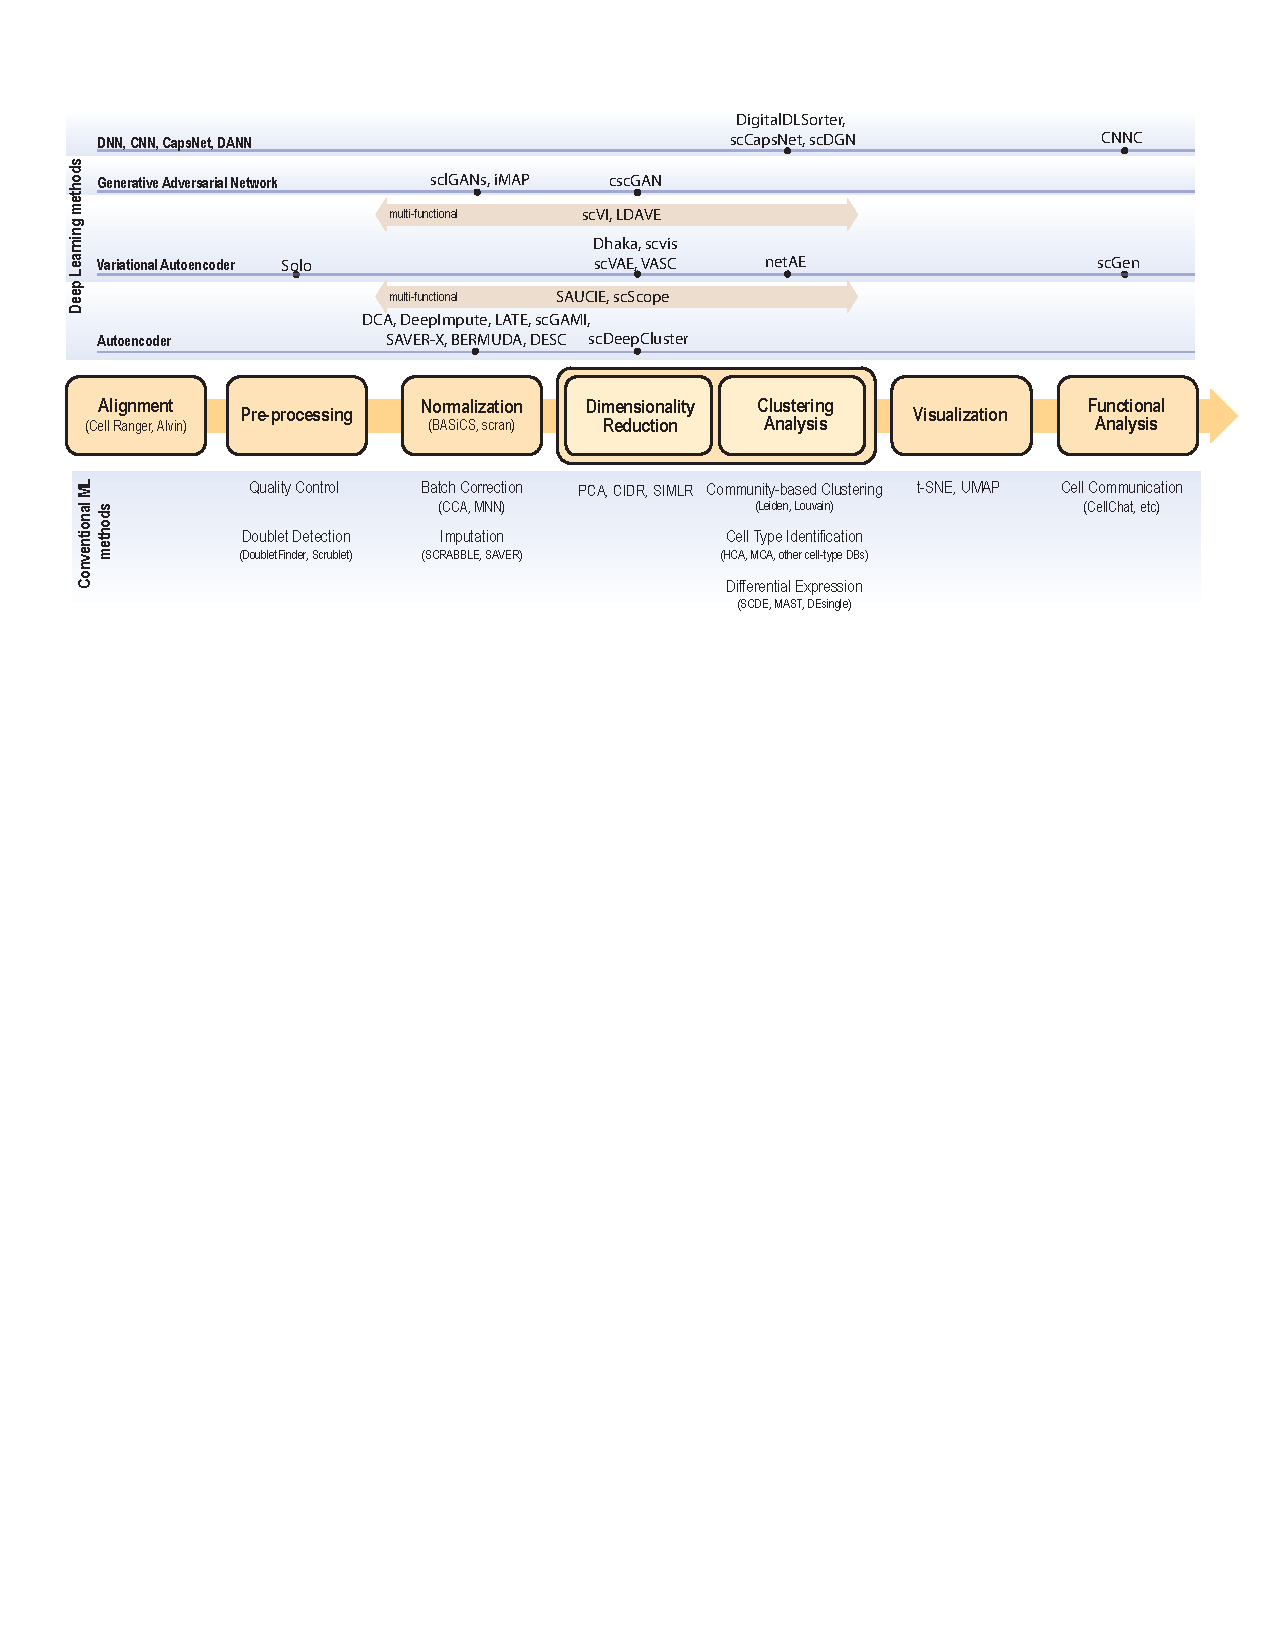
\includegraphics[width=22.31in]{Figures/Figure1} 

}

\caption{Single cell data analysis steps for both conventional ML methods (bottom) and DL methods (top). Depending on the input data and analysis objectives, major scRNA-se analysis steps are illustrated in the center flow chart. The convential ML approaches along with optional analysis modules are presented below each analysis step. Deep learning approaches are categorized as neural network models (DNN, CNN, CapsNet, and DANN), Generalive Adversarial Network (GAN), Variational Autoencoder, and Autoencoder. For each DL approach, optional algorithms are listed on top of each step in the pipeline.}\label{fig:Figure1}
\end{figure}

With the advantage of identifying each cell and unique molecular identifiers (UMIs) for expressions of each gene in a single cell, scRNA-seq data are embedded with increased technical noise and biases {[}23{]}. Quality control (QC) is the first and the key step to filter out dead cells, double-cells, or cells with failed chemistry or other technical artifacts. The most commonly adopted three QC covariates include the number of counts (count depth) per barcode identifying each cell, the number of genes per barcode, and the fraction of counts from mitochondrial genes per barcode \citep{RN81}.

\textbf{Normalization} is designed to eliminate imbalanced sampling, cell differentiation, viability, and many other factors. Approaches tailored for scRNA-seq have been developed including the Bayesian-based method coupled with spike-in, or BASiCS \citep{RN97}, deconvolution approach, scran \citep{RN89}, and sctransfrom in Seurat where regularized Negative Binomial regression was proposed \citep{RN83}. Two important steps, batch correction and imputation, will be carried out if required by the analysis:

\begin{itemize}
\item
  \textbf{Batch Correction} is a common source of technical variation in high-throughput sequencing experiments due to variant experimental conditions such as technicians and experimental time, imposing a major challenge in scRNA-seq data analysis. Batch effect correction algorithms include detection of mutual nearest neighbors (MNNs) \citep{RN84} , canonical correlation analysis (CCA) with Seurat \citep{RN79}, and Hormony algorithm through cell-type representation \citep{RN74}.
\item
  \textbf{Imputation} step is necessary to handle high sparsity data matrix, due to missing value or dropout in scRNA-seq data analysis. Several tools have been developed to ``impute'' zero values in scRNA-seq data, such as SCRABBLE \citep{RN29}, SAVER \citep{RN30} and scImpute \citep{RN31}.
  Dimensionality reduction and visualization are essential steps to represent biological meaningful variation and high dimensionality with significantly reduced computational cost. Dimensionality reduction methods, such as PCA, are widely used in scRNA-seq data analysis to achieve that purpose. More advanced nonlinear approaches that preserve the topological structure and avoid overcrowding in lower dimension representation, such as LLE \citep{RN32} (used in SLICER \citep{RN33}), tSNE \citep{RN34}, and UMAP \citep{RN35} have also been developed and adopted as a standard in single-cell data visualization.
\end{itemize}

\textbf{Clustering analysis} is a key step to identify cell subpopulations or distinct cell types to unravel the extent of heterogeneity and their associated cell-type-specific markers. Unsupervised clustering is frequently used here to categorize cells into clusters by their similarity often taken the aforementioned dimensionality-reduced representations as input, such as community detection algorithm Louvain \citep{RN36} and Leiden \citep{RN37}, or data-driven dimensionality reduction followed with k-Means cluster by SIMLR \citep{RN38}.

\textbf{Feature selection} is another important step in single-cell RNA-seq analysis is to select a subset of genes, or features, for cell-type identification and functional enrichment of each cluster. This step is achieved by differential expression analysis designed for scRNA-seq, such as MAST that used linear model fitting and likelihood ratio testing \citep{RN40}; SCDE that adopted a Bayesian approach with a Negative Binomial model for gene expression and Poisson process for dropouts \citep{RN41}, or DEsingle that utilized a Zero-Inflated Negative Binomial model to estimate the dropouts \citep{RN42}.

Besides these key steps, downstream analysis can include cell type identification, coexpression analysis, prediction of perturbation response, where DL has also been applied. Other advanced analyses including trajectory inference and velocity and pseudotime analysis are not discussed here because most of the approaches on these topics are non-DL based.

\hypertarget{ch-3}{%
\chapter{Overview of common deep learning models for scRNA-seq analysis}\label{ch-3}}

\begin{figure}

{\centering 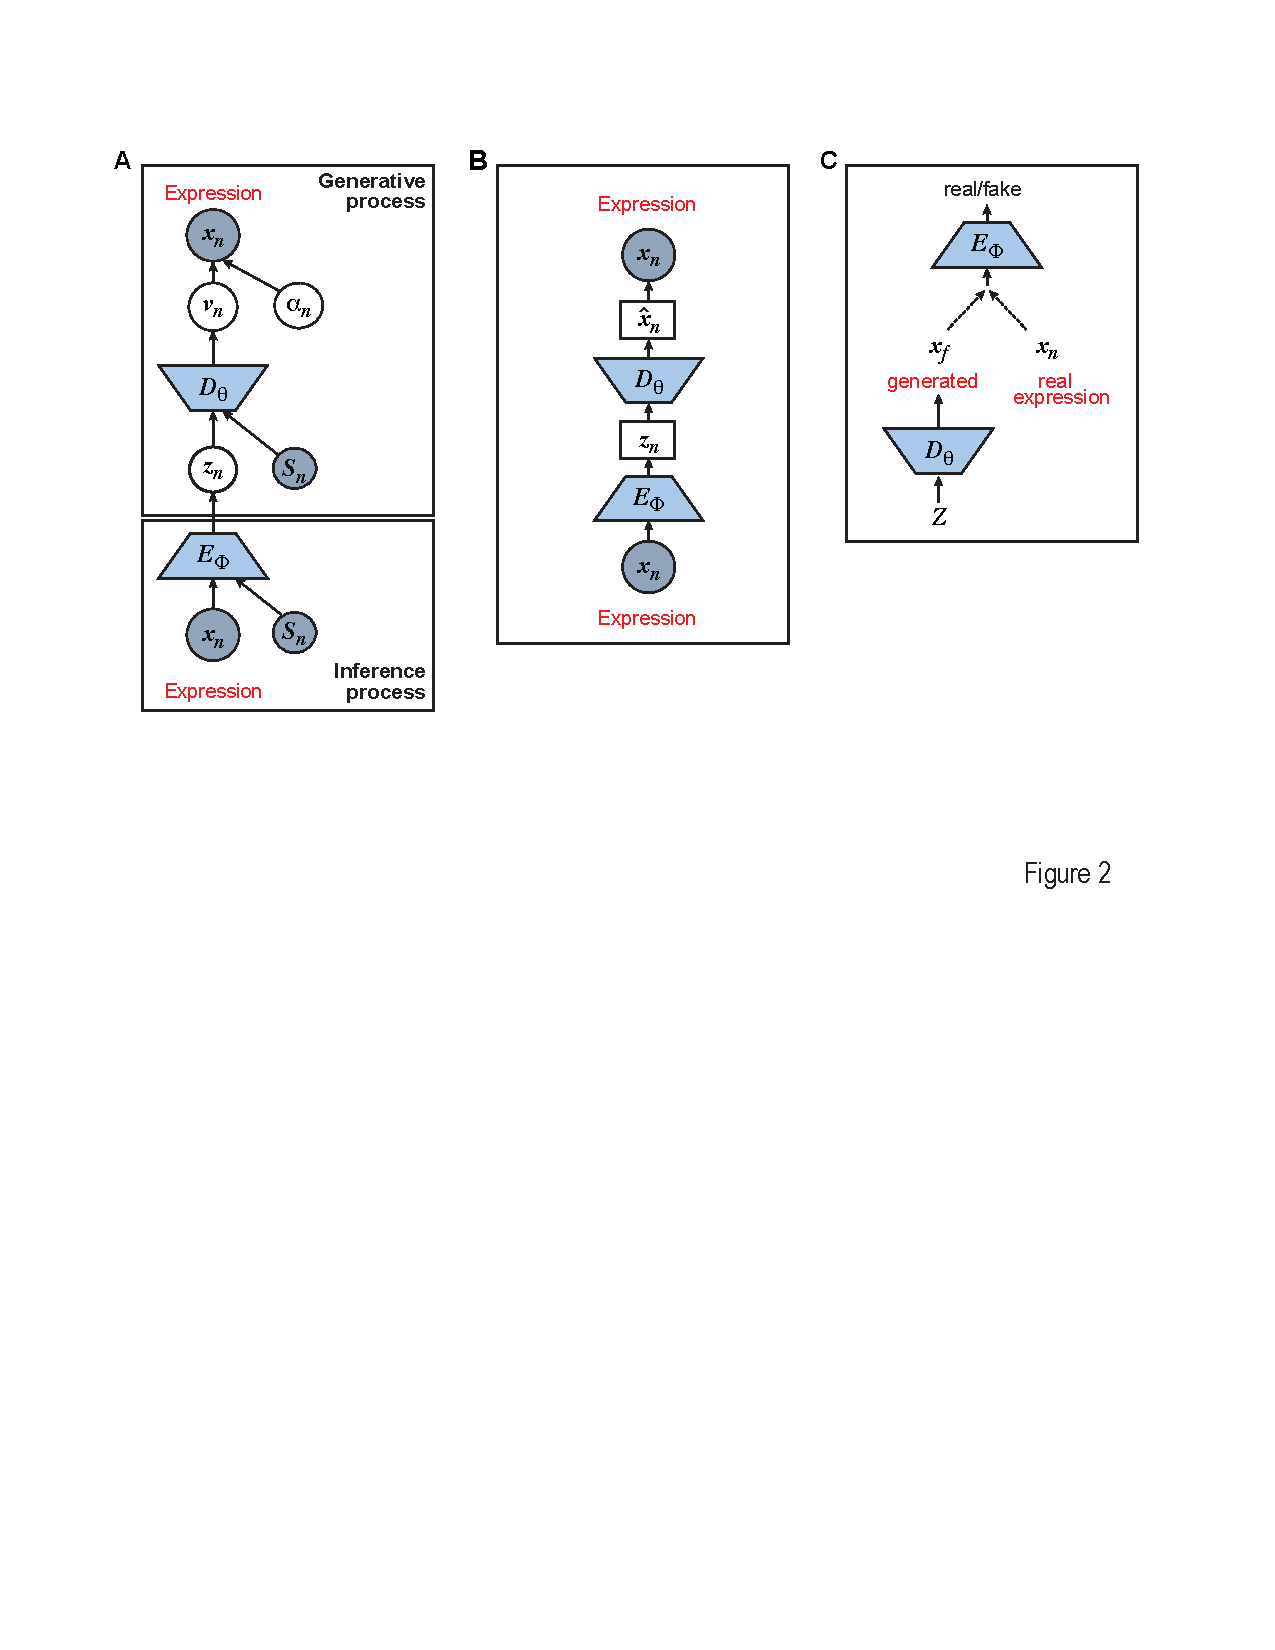
\includegraphics[width=21.28in]{Figures/Figure2} 

}

\caption{Graphical models of the surveyed DL models including A) Variational Autoencoder (VAE); B) Autoencoder (AE); and C) Generative Adversarial Network (GAN)}\label{fig:Figure2}
\end{figure}

Unsupervised learning is the key step in the scRNA-Seq analysis, including batch correction, dimension reduction, imputation, and clustering, which lend themselves naturally to unsupervised DL models including the variational autoencoder (VAE), the autoencoder (AE), or generative adversarial networks (GAN). Also, adversarial transfer learning has been applied for cell-type classification. We started our review by introducing the general formulations of VAE, AE, and GAN for scRNA-seq together with their training strategies. These general formulations facilitate understanding the methodologies used by different papers in developing their specific algorithms, enabling us to focus on the different features of each method and bring attention to their uniqueness and novelty.

\hypertarget{ch-3-1}{%
\section{Variational Autoencoder (VAEs) for scRNA-Seq data}\label{ch-3-1}}

Let \(x_{n}\) represent a \(G \times 1\) vector of gene expression (UMI counts or normalized, log-transformed expression) of \(G\) genes in cell n, where \(x_{gn}\) denotes gene \(g\)'s expression, which is assumed to follow some distribution \(p(x_{gn} \vert v_{gn}, \alpha_{gn} )\) (e.g., zero-inflated negative binomial (ZINB) or Gaussian), where \(v_{gn}\) and \(\alpha_{gn}\) are parameters of the distribution (e.g., mean, variance, or dispersion) (Fig.\ref{fig:Figure2}A). We consider the first parameter \(v_{gn}\) to be of particular interest (e.g., the mean counts) for the scRNA-seq analysis and is thus further modeled as a function of a d-dimension latent variable \(z_{n} \in R^{d}\) and an observed variable \(s_{n}\) (e.g., the batch ID) by a decoder neural network \(D_{\theta}\) (Fig.\ref{fig:Figure2}A) as

\begin{equation}
v_{n} = D_{\theta}(z_{n}, s_{n}) \label{eq:eq1}
\end{equation}

where the \(g\)th element of \(v_{n}\) is \(v_{gn}\) and \(\theta\) is a vector of decoder weights, \(z_{n}\) represents a low-dimensional latent representation of gene expression and is used in all the works for visualization and clustering. For VAE, \(z_{n}\) is commonly assumed to follow a multivariate standard normal prior, i.e., \(p(z_{n})=N(0,I_{d})\) with \(I_{d}\) being a \(d \times d\) identity matrix. The second parameter \(\alpha_{gn}\) of \(p(x_{gn} \vert v_{gn}, \alpha_{gn})\) is a nuisance parameter, which is assumed with a prior distribution \(p(\alpha_{gn})\) and can be either estimated or marginalized in variational inference. Now define \(\Theta=\{\theta, \alpha_{ng}\forall{n},g\}\) as the collection of the unknown model parameters. Then, \(p(x_{gn} \vert v_{gn}, \alpha_{gn})\) and (\eqref{eq:eq1}) together define the likelihood \(p(x_{gn} \vert z_{n}, s_{gn}, \Theta)\).

The goal of training or inference is to compute the maximum likelihood estimate of \Theta 

\begin{equation}
    \hat{\Theta}_{ML} = argmax_{\Theta}\sum_{n=1}^{N}\log(x_{n} \vert s_{n},\Theta) \approx argmax_{\Theta}\sum_{n=1}^{N}\textit{L}(\Theta) \label{eq:eq2}
\end{equation}

where \(p(x_{n}\vert s_{n},\Theta)=\int(p(x_{n} \vert z_{n}, s_{n}, \Theta)p(z_{n})\textit{d}z_{n}\) is the marginal likelihood, which is in general analytically intractable but can be lower-bounded by the evidence lower bound (ELBO) \(\textit{L}(\Theta)\), expressed as

\begin{equation}
  \textit{L}(\Theta) = E_{q(z_{n} \vert x_{n},s_{n}, \Theta)}[\log{p(x_{n}\vert z_{n},s_{n}, \Theta)}] - D_{KL}[q(z_{n}\vert x_{n},s_{n},\Theta)\|p(z_{n})] \label{eq:eq3}
\end{equation}

where \(q(z_{n}│x_{n},s_{n})\) is an approximate to the intractable posterior distribution \(p(z_{n}\vert x_{n},s_{n})\). To make the variational inference tractable \(q(z_{n}\vert x_{n},s_{n})\) is assumed in most cases as a multivariate Gaussian

\begin{equation}
  q(z_{n} \vert x_{n},s_{n})= N(\mu_{z_{n}},diag({\sigma_{Z_{n}}}^2)) \label{eq:eq4}
\end{equation}

whose means and variances \({\mu_{z_{n}},{\sigma_{Z_{n}}}^2}\) are given by an encoder network \(E_{\phi}\) applied to \(x_{n}\) and \(s_{n}\) (Fig.\ref{fig:Figure2}A) as

\begin{equation}
   {\mu_{z_{n}},{\sigma_{Z_{n}}}^2} = E_{\phi}(x_{n},s_{n}) \label{eq:eq5}
\end{equation}

where \pi is the vector of the unknown decoder weights. Because of the approximation by \(\textit{L}(\Theta)\) in (\eqref{eq:eq2}) and the introduction of the decoder network in eq.\eqref{eq:eq4}, the model parameters to be estimated become \(\theta=\{ \theta,\phi, \alpha_{ng}, \forall{n}, g \}\). Optimization of \(\textit{L}(\Theta)\) in (\eqref{eq:eq2}) is computed efficiently by stochastic optimization, where the gradient is calculated by backpropagation.

All the surveyed papers that deploy VAE follow this general modeling process. However, an alternative and more general formulation treats it as optimization with a loss function expressed as

\begin{equation}
L(\Theta) = - L(\Theta) + \sum_{k=1}^{K}\lambda_{k}L_{k}(\Theta)\label{eq:eq6}
\end{equation}

where \(L_{k}\forall{k}=1,…,K\) are \(K\) additional function-specific losses introduced to constrain the model for different functions (clustering, cell type prediction, etc), and \(\lambda_{k}\)s are the Lagrange multipliers. With this general formulation, for each paper, we focus on the survey the specific choice of data distribution \(p(x_{gn} \vert v_{gn},\alpha_{gn})\) that defines \(L(\Theta)\), different \(L_{k}\) designed for specific functions, and how the decoder and encoder are applied to model different aspects of scRNA-seq data.

\hypertarget{ch-3-2}{%
\section{Autoencoders (AEs) for scRNA-seq data}\label{ch-3-2}}

AEs have been proposed to learn the low dimensional latent representation of expression \(x_{n}\). The AE includes an encoder \(E_{\phi}\) and a decoder \(D_{\theta}\) (Fig.\ref{fig:Figure2}B) such that

\begin{equation}
    z_{n}=E_{\phi}(x_{n}); \hat{x_{n}} = D_{\theta}(z_{n})  \label{eq:eq7}
\end{equation}

where like VAE \(z_{n} \in R^{d}\) is the d-dimension latent variable, \(\Theta = \{\theta,\phi\}\) are encoder and decoder weight parameters, and \(\hat{x_{n}}\) defines the parameters (e.g.~mean) of data distribution and thus the likelihood \(p(x_{n} \vert \Theta)\) (Fig.\ref{fig:Figure1}B). Note that the mean of \(p(x_{n}\vert \Theta)\) is often considered as the imputed and denoised expression of \(x_{n}\). For most common AEs, \(p(x_{n}\vert \Theta)\) assumes a Gaussian distribution and \(\hat{x_{n}}\) becomes the mean of the Gaussian and can be directly used as imputed, normalized gene expression. Nevertheless, additional designs can be introduced to attend imputation specifically. \(p(x_{n}\vert \Theta)\) can also be negative binomial (NB) or ZINB as in DCA \citep{RN80} to model the reads count directly with their parameters defined as functions of \(\hat{x_{n}}\). Additional design can be included in the AE model for batch correction, clustering, and other functions.

The training of the AE is generally carried out by stochastic gradient descent algorithms to minimize the loss with the general expression similar to that of VAE in eq.\eqref{eq:eq6}

\begin{equation}
    L(\Theta)=L_{0}(\Theta)+\sum_{k=1}^{K}\lambda_{k}L_{k}(\Theta) \label{eq:eq8}
\end{equation}

where \(L_{0}\) is \(-\log{p(x_{n}\vert \Theta)}\), and \(L_{k}s\) are \(K\) additional function-specific losses. When \(p(x_{n} \vert \Theta)\) is the Gaussian, \(L_{0}\) becomes one of the most commonly used mean square error (MSE) loss

\begin{equation}
L_{0}(\Theta)=\sum_{n=1}^{N}\|x_{n}-\hat{x_{n}}\|_{2}^{2} \label{eq:eq9}
\end{equation}

Because different AE models differ in their AE architectures and the loss functions, we will discuss the specific architecture and the loss functions for each reviewed model.

\hypertarget{ch-3-3}{%
\section{Generative adversarial networks (GANs) for scRNA-seq data}\label{ch-3-3}}

GANs have been used for imputation, data generation and augmentation of the scRNA-seq analysis. Without loss of generality, the GAN, when applied to scRNA-seq, is designed to learn to generate gene expression profiles from \(p_{x}\), the distribution of \(x_{n}\), the count or normalized expression vectors of the scRNA data. The vanilla GAN consists of two deep neural networks \citep{RN98}. The first network is the generator \(G_{\theta}(z_{n},y_{n})\) with parameter \(\theta\), which is essentially a decoder that takes a noise vector \(z_{n}\) from the distribution \(p_{z}\) and a class label \(y\) (e.g.~cell type) as input and is trained to generate \(x_{f}\), a ``fake'' sample of a gene expression profile (Fig.\ref{fig:Figure2}C). Note that including a class label \(y_{n}\) at the input is optional and when it is included, the model is known as the conditional GAN. The second network is the discriminator network \(D_{\phi_{D}}\) with parameters \(\phi_{D}\), which is a classifier trained to distinguish between the ``real'' sample \(x\) and fake data \(x_{f}\) (Fig.\ref{fig:Figure1}C). The generator \(G_{\theta}\) and discriminator \(D_{\phi_{D}}\) are trained to outplay each other, resulting in a minimax game, in which \(G_{\theta}\) is forced by \(D_{\phi_{D}}\) to produce better samples, which, when converge, can fool the discriminator \(D_{\phi_{D}}\), thus becoming samples from \(p_{x}\). The vanilla GAN suffers heavily from training instability and mode collapsing \citep{RN104}. To that end, Wasserstein GAN (WGAN) was developed to effectively improve the training stability and convergence \citep{RN107}. The WGAN loss computes the Wasserstein distance, also called the earth moving distance between the real and fake sample distributions \citep{RN181}:

\begin{equation}
  L(\Theta)=\max_{\phi_{D}}\sum_{n=1}^{N}D_{\phi_{D}}(x_{n})-\sum{n=1}^{N}D_{\phi_{D}}(G_{\theta}(z_{n},y_{n})) \label{eq:eq10}
\end{equation}

Additional terms can also be added to (\eqref{eq:eq10}) to constrain the functions of the generator. Training based on the WGAN loss in Eq. (\eqref{eq:eq10} ) amounts to a min-max optimization, which iterates between the discriminator and generator, where each optimization is achieved by a stochastic gradient descent algorithm through backpropagation. The WGAN requires D to be K-Lipschitz continuous \citep{RN104}, which can be satisfied by adding the gradient penalty to the WGAN loss \citep{RN103}. Once the training is done, the generator \(G_{\phi_{G}}\) can be used to generate gene expression profiles of new cells.

\hypertarget{ch-4}{%
\chapter{Overview of datasets and evaluation metrics}\label{ch-4}}

A variety of datasets and performance evaluation metrics have been used to demonstrate the performance of the surveyed DL models for different tasks. We summarize these datasets and evaluation metrics in Table \ref{fig:Table2a} \& \ref{fig:Table3}. We detail the mathematical definition of the evaluation metrics in the following.

\hypertarget{ch-4-1}{%
\section{Evaluation methods}\label{ch-4-1}}

An extensive list of evaluation methods has been proposed for different scRNA-seq analysis tasks \citep{RN44, RN45, RN43}. We provide an overview here the methods adopted in the surveyed papers. We discuss them according to the key categories on which the surveyed papers are organized, namely, imputation, batch effect correction, dimension reduction and clustering, cell type identification, and functional analysis.

\hypertarget{ch-4-1-1}{%
\subsection{Imputation}\label{ch-4-1-1}}

The evaluation of the performance of imputation methods considers their ability to recover biological signals and improve downstream analyses. For this two main methods have been used. First is the evaluation of similarity between bulk and imputed scRNA-seq data. Second is the evaluation of imputation on unsupervised clustering.

The first approach consist in assessing the similarity between bulk and imputed scRNA-seq data. For a given scRNA-seq dataset, the ``pseudobulk'', or the average of normalized (log2-transformed) scRNA-seq counts across cells, is calculated first, and the Spearman's rank correlation coefficient (SCC) between the pseudobulk and the bulk RNA-seq profile of the same cell type is evaluated. The statistical significance is assessed whether SCCs bewteen the bulk and pseudobulks from two imputation methods are equal.

The second approach consist in measuring the accuracy of several clustering assignments methods using four metrics:

\begin{itemize}
\tightlist
\item
  Entropy of accuracy (\(H_{acc}\)) and entropy of purity (\(H_{pur}\)). Hacc (\(H_{pur}\)) measures the diversity of the ground-truth labels (predicted cluster labels) within each predicted cluster group (ground-truth group), respectively.
\end{itemize}

\[H_{acc}=-1\frac{1}{M}\sum_{i=1}^{M}\sum_{j=1}^{N_{i}}p_{i}(x_{j})\log{p_{i}(x_{j})}\]

\[H_{pur}=-1\frac{1}{N}\sum_{i=1}^{N}\sum_{j=1}^{M_{i}}q_{i}(x_{j})\log{q_{i}(x_{j})}\]

where \(M\) is the total number of predicted clusters from the clustering algorithm, \(N\) is the number of ground-truth clusters, \(M_{i}\), (or \(N_{i}\)) is the number of predicted clusters (or ground-truth clusters) in the ith ground -truth cluster (or predicted cluster), respectively. \(p_{i}(x_{j})\) (or \(q_{i}(x_{j}))\) are the proportions of cells in the \(j\)th ground-truth cluster (or predicted cluster) relative to the total number of cells in the \(i\)th predicted cluster (or ground-truth clusters), respectively. A smaller value of \(H_{acc}\) means the cells in a predicted cluster are constantly labeled from the same ground-truth group, while A smaller value of \(H_{pur}\) means the cells in the ground-truth groups are homogeneous with the same predicted cluster labels \citep{RN44}. However, smaller \(H_{acc}\) (or \(H_{pur}\) ) can lead to over-clustering (or under-cluster), when each predicted cluster contains 1 cell (\(H_{acc}\) = 0) or all cells in one predicted cluster (\(H_{pur}\) = 0).

\begin{itemize}
\tightlist
\item
  Adjusted Rand index (ARI). Rand index (RI) is another measure of constancy between two clustering outcomes. If \(a\) (or \(b\)) is the count of number of pairs of cells in one cluster (or different clusters) from one clustering algorithm but also fall in the same cluster (or different clusters) from the other clustering algorithm, then, \(RI=(a+b)/{\binom{n}{2}}\), where \(\binom{n}{2}\) is the total number of pairs when given n cells. The RI has a value between 0 and 1, with 0 indicating that the two clustering algorithms do not agree on any pair of cells and 1 indicating that the two clustering algorithms are exactly the same. ARI is a corrected-for-chance version of \(RI\), or
\end{itemize}

\[ARI = \frac{RI-E[RI]}{\max(RI)-E[RI]}\]
where \(E[RI]\) is the expected Rand Index \citep{RN107}.

\begin{itemize}
\tightlist
\item
  Median Silhouette index. The Silhouette index is defined as
\end{itemize}

\[ s(i)=\frac{b(i)-a(i)}{\max(a(i),b(i))}\]

where \(a(i)\) is the average dissimilarity of \(i\)th cell to all other cells in the same cluster, and \(b(i)\) is the average dissimilarity of \(i\)th cell to all cells in the closest cluster. The range of \(s(i)\) is {[}−1,1{]}, with 1 to be well-clustered with appropriate labels, and -1 to be completely misclassified. \(s(i) = 0\) indiates the cell could be assigned to nearest clusters (or overlapping clusters).

A good imputation method should allow perform downstream (clustering) analyses without introducing any artifacts or false signals.

\hypertarget{ch-4-1-2}{%
\subsection{Batch effect correction}\label{ch-4-1-2}}

When evaluating the performance of a batch correction method, we need to consider how well it mixes the shared cell types between different batches and at the same time identifies batch-specific cells. The existing metrics can be classified as cluster-level and cell-level metrics. Cluster level metrics are those used for evaluating clustering performance and include adjusted rand index (ARI), normalized mutual information (NMI), and silhouette coefficients. They are easy to compute but do not measure local mixture of cells from different batches. This drawback is addressed by the cell-level metrics, which includes k-nearest neighbor batch-effect test (kBET), local inverse Simpson's index (LISI), and classifier-based. Because the cluster-level metrics will be discussed in detail in Section \ref{ch-4-2-3}, we focus on discussing cell-level metrics in this section.

Entropy of mixing. This metric evaluates the mixing of cells from different batches in the neighborhood of each cell \citep{RN84}. It first randomly sample N cells and then for each cell it calculates the regional entropy of mixing as

\[E = \sum_{i=1}^{C}p_{i}\log{(p_{i})}\]

where \(C\) is the number of batches and \(p_{i}\) is the proportion of cells from batch \(i\) among \(N\) nearest cells (e.g.~\(N\) = 100). The total entropy is the sum of reginal entropies. The computation repeats \(K\) times to obtain an empirical distribution of the entropy of mixing.

\textbf{Maximum Mean Discrepancy (MMD)} is a non-parametric distance between distributions based on the reproducing kernel Hilbert space (RKHS) \citep{RN185}, or, MMD is a distance-based measure between two distribution \(p\) and \(q\) based on the mean embeddings \(\mu_{p}\) and \(\mu_{q}\) in a reproducing kernel Hilbert space \(F\),

\[MMD(F,p,q)=\sup_{f \in F}\|\mu_{p}-\mu_{q}\|_{f}\]

MMD will vanish for most finite samples \(x_{k}\) and \(y_{k}\) only if two distributions are the same.

\textbf{k-Nearest neighbor batch-effect test (kBET)}. kBET assesses the batch mixing by comparing the batch-specific distribution within \(k\)-nearest neighbors (kNNs) of a cell with the global distribution of batches \citep{RN105}. It uses a \(X^2\)-based test for random neighborhoods of fixed size to determine whether they are well mixed. Given a dataset of \(N\) cells from \(L\) batches with \(N_{l}\) denoting the number of cells in batch \(l\). Under the null hypothesis that cells are `well mixed', that is the absence of batch effect, we have the test statistics as

\[a_{n}^{k} = \sum_{l=1}^{L}\frac{(N_{nl}^{k}-k*f_{l})^{2}}{k*f_{l}} \sim X^{2}_{L-1}\]

where \(N_{nl}^{k}\) is the number of cells from batch \(l\) in the \(k\)-nearest neighbors of cell \(n\), \(f_{l}\) is the global fraction of cells in batch \(l\), or \(f_{l}=\frac{N_{l}}{N}\), and \(X_{L-1}^2\) denotes the \(X^2\) distribution with \(L-1\) degrees of freedom. The averaged rejection rate of the \(Χ^2\) test for all cells is used to define the performance of a batch correction method.

\textbf{Local Inverse Simpson's Index (LISI).} Like kBET, LISI also compares the batch mixing at local level with global batch distribution. However, unlike kBET, which is agnostic of cell types, LISI requires well mixing of cells from the same cell type but not of those from different types \citep{RN74}. LISI evaluates cell-type-specific mixing using an inverse Simpson's Index in a local neighborhood of each cell. LISI builds Gaussian kernel-based distributions of local neighborhoods sensitive to local diversity. It calculates inverse Simpson's Index in the k-nearest neighbors of cell \(n\) for all batches as \(\frac{1}{\lambda(n)}=\frac{1}{\sum_{l=1}^{L}(p(l))^{2}}\), where \(p(l)\) denotes the proportion of batch \(l\) in the \(k\)-nearest neighbors. The score reports the effective number of batches in the \(k\)-nearest neighbors of cell \(n\). Inverse Simpson's Index in the \(k\)-nearest neighbors of cell \(n\) can also be calculated to evaluate the diversity of different cell types. However, in an ideal case, LISI score should be 1, reflecting a separation of unique cell types.

\textbf{Classifier-based.} Although LISI addresses the issue of cell-type proportion of different batches but it is hard to summarize all single cell-level LISI scores into a simple statistic for comparing across different methods \citep{RN53}. The classifier-based approach addresses this issue by using two distinct local classifiers for each single cell. The first classifier classifies every single cell as positive and negative cells. A single cell \(n\) is positive if at least 50\(%
\) cells of its k-nearest neighbor (KNN) cells are from the same cell-type label, otherwise `negative'. The positive cells are further classified into true and false positive cells, where true positive cells are those surrounded by appropriate portions of cells with L batches. In other words, if we sample \(k\) cells from this cell-type cluster, the expected number of cells from batch \(l\) will be \(k*f_{l}\), where \(f_{l}\) is the global fraction of cells in batch \(l\). A positive cell in this cluster is a true positive when the observed cell numbers for each batch among its \(k\) neighbors are within 3 standard deviations around the expected numbers. The proportions of positive cells and true positive cells are used as the summary metrics to evaluate the overall performance of batch effect removal. The higher the proportions, the better the algorithm.

\hypertarget{ch-4-1-3}{%
\subsection{Clustering}\label{ch-4-1-3}}

Evaluating the performance of clustering algorithms is not as trivial as counting the number of errors like supervised learning. In general, the clustering performance evaluation metric should not just take absolute corrected labelled cells into account but also consider if the clustering defines a good similarity or separation in the dataset compared to ground truth. When ground truth is not available, evaluation must be performed using model itself such as clustering distance, dispersion, etc. Similar measures, such as Adjusted Rand Index (ARI) and Silhouette Index discussed in Section \ref{ch-4-2-1} can also be employed here to measure the agreement between predicted assignment to the ground-truth assignment.

\textbf{Normalized Mutual Information (NMI).} The mutual information(MI) {[}47{]} is a measure of mutual dependency between two cluster assignments \(U\) and \(V\). It quantifies the amount of information we could have about one assignment by observing the other assignment. For \(N\) samples, we have the entropy for cluster assignments \(U\) and \(V\) as

\[H(U)=\sum_{i=1}^{\vert U \vert}P_{U}(i)\log{(P_{U}(i))},  H(V)=\sum_{i=1}^{\vert V \vert}P_{V}(i)\log{(P_{V}(i))}\]

where \(P_{U}(i)=\frac{\vert U_{i} \vert}{N}\) and \(P_{V}(j)=\frac{\vert V_{j} \vert}{N}\). Also, define the joint distribution probability is \(P_{UV}(i,j)=\frac{\vert U_{i}\cap V_{j} \vert}{N}\). Then, the mutual information of \(U\) and \(V\) is defined as

\[MI(U,V)=\sum_{i=1}^{\vert U \vert}\sum_{j=1}^{\vert V \vert}P_{UV}(i,j)\log{\frac{P_{UV}(i,j)}{P_{U}(i)P_{V}(j)}}\]

The NMI is a normalization of the \(MI\) score between 0 and 1. For example, the average NMI is defined as \citep{RN250}

\[NMI(U,V)=\frac{2 \times MI(U,V)}{[H(U) + H(V)]}\]

\textbf{Homogeneity, Completeness, and V-Measure.} The homogeneity score (HS) measures the extent to which its clusters contain only samples that belong to one cell type, or \(HS=1-H(P(U\vert V))/H(P(U))\), where \(H()\) is the entropy, and \(U\) is the ground-truth assignment and \(V\) is the predicted assignment. The \(HS\) range from 0 to 1, where 1 indicates perfectly homogeneous labelling. Similarly, the completeness score (CS) is defined as \(CS=1-H(P(V \vert U))/H(P(V))\), its values range from 0 to 1, where 1 indicates all member from a ground-truth label are assigned to a single cluster.

The V-Measure {[}54\emph{(Reference Not Found)}{]} is the harmonic mean between \(HS\) and \(CS\), defined as \(V_{\beta}=\frac{(1+\beta)HS×CS}{\beta HC+CS}\), where \(\beta\) indicates the weight of \(HS\). V-Measure is a more symmetric, i.e.~switching the true and predicted cluster labels does not change V-Measure.

\hypertarget{ch-5}{%
\chapter{Survey of deep learning models for scRNA-Seq analysis}\label{ch-5}}

In this section, we survey applications of DL models for scRNA-seq analysis. To better understand the relationship between the problems that each surveyed work addresses and the key challenges in the general scRNA-seq processing pipeline, we divide the survey into sections according to steps in the scRNA-seq processing pipeline illustrated in Fig.\ref{fig:Figure1}. For each DL model, we present the model details under the general model framework introduced in Section \ref{ch-3} and discuss the specific loss functions. We also survey the evaluation metrics and summarize the evaluation results. To facilitate cross-references of the information, we summarized all algorithms reviewed in this section in Table \ref{fig:Table1} and tabulate the datasets and evaluation metrics used in each paper in Tables \ref{fig:Table2a} \& \ref{fig:Table3}. We also listed all other algorithms that each surveyed method evaluated against in Fig.\ref{fig:Figure3}, highlighting the extensiveness these algorithms were assessed for their performance.

\begin{figure}

{\centering 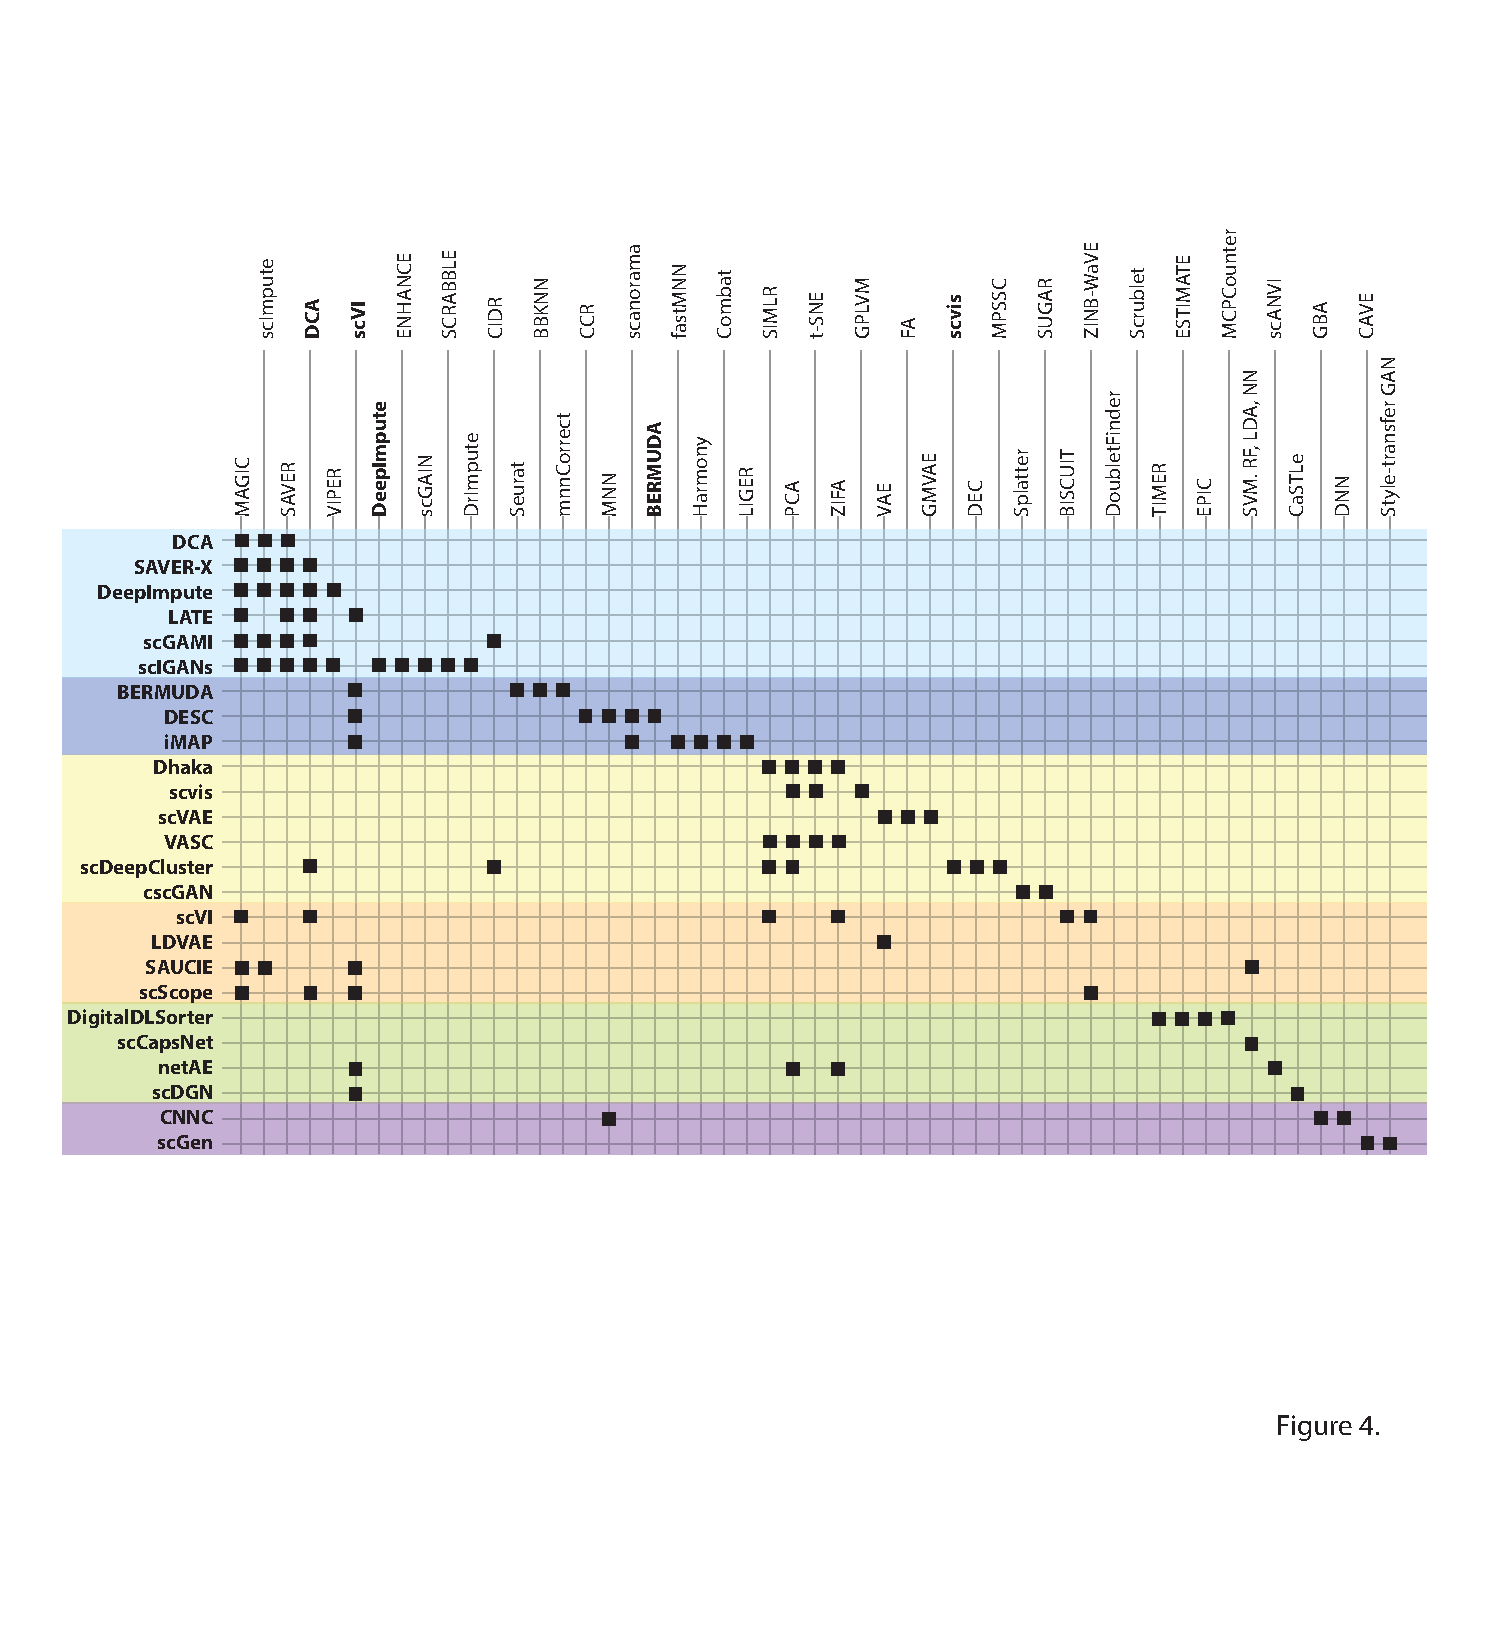
\includegraphics[width=26.19in]{Figures/Figure3} 

}

\caption{Add figure caption here}\label{fig:Figure3}
\end{figure}

\hypertarget{ch-5-1}{%
\section{Imputation}\label{ch-5-1}}

The goal of imputation is to estimate the missing gene expression values due to dropout, or the failure to amplify the original RNA transcripts. These missing expression values can affect downstream bioinformatics analysis significantly as it decreases the power of the studies and introduces biases in gene expression \citep{RN46}. VAE, AE, and GAN have been applied for imputation and we review their specific model designs in this section.

\hypertarget{ch-5-1-1}{%
\subsection{DCA:deep count autoencoder}\label{ch-5-1-1}}

DCA \citep{RN53} is an AE designed for imputation (Fig.\ref{fig:Figure2}-B. DCA is implemented in Python as a command line and also integrated into the Scanpy framework.

\emph{Model.} DCA models UMI counts of a cell with missing values using the ZINB distribution as

\begin{equation}
p(x_{gn} \vert \Theta)=\pi_{gn}\delta(0)+(1-\pi_{gn})NB(v_{gn},\alpha_{gn}),\space for\space g=1,…G; n=1,…N \label{eq:eq11}
\end{equation}

where \(\delta(⋅\)) is a Dirac delta function,\(NB(,)\) denotes the negative binomial distribution and \(\pi_{gn},v_{gn}, \space and \space \alpha_{gn}\) are dropout rate, mean, and dispersion, which are functions of DCA decoder output \(\bf{\hat{x}_{n}}\) as

\begin{equation}
\bf{\pi_{n}}=sigmoid(\bf{W_{\pi}\hat{x}_{n}}); \bf{v_{n}}=exp(\bf{W_{v}\hat{x}_{n}}); \bf{\alpha_{n}}=exp(\bf{W_{\alpha}\hat{x}_{n}}) \label{eq:eq12}
\end{equation}

where the \(g\)th element of \(\bf{\pi_{n}}\), \(\bf{v_{n}}\), and \(\bf{\alpha_{n}}\) are \(\pi_{gn}\) and \(\alpha_{gn}\), respectively and \(\bf{W_{\pi}}\), \(\bf{W_{v}}\), and \(\bf{W_{\alpha}}\) are additional weights to be estimated.
The DCA encoder and decoder follow the general AE formulation as in Eq. (\eqref{eq:eq7}) but the encoder takes the size factor normalized, log-transformed expression as input.
The encoder and decoder architecture are the conventional deep neural networks.
The parameters to be trained are \(\Theta=\{\theta,\phi,W_{\pi},W_{v},W_{\alpha}\}\).
To train the model, DCA uses a constrained log-likelihood as the loss function as

\begin{equation}
L(\Theta)=\sum_{n=1}^{N} \sum_{g=1}^{G} (-logp(x_{gn}\vert \Theta) + \lambda\pi^{2}_{gn} ) \label{eq:eq13}
\end{equation}

where the second term functions as a ridge prior on the dropout probabilities.
Once the DCA is trained, the mean counts \(v_{n}\) are used as the denoised and imputed counts for cell \(n\).

\emph{Evaluation metrics.} A Density Resampled Estimate of Mutual Information (DREMI) measure was adapted for the higher dimensionality and sparsity of scRNA-seq data.

\emph{Results.} For evaluation, DCA is compared to other methods using simulated data (using Splatter R package), and a real bulk transcriptomics data from a developmental C. elegans time-course experiment was used with added simulating single-cell specific noise. For this. gene expression was measured from 206 developmentally synchronized young adults over a twelve-hour period (C elegans). Single-cell specific noise was added in silico by genewise subtracting values drawn from the exponential distribution such that 80\(%
\) of values were zeros. The paper analyzed the Bulk contains less noise than single-cell transcriptomics data and can thus aid in evaluating single-cell denoising methods by providing a good ground truth model. The authors also did a comparison of other methods like SAVER \citep{RN30}, scImpute \citep{RN31}, and MAGIC \citep{RN111}. DCA denoising recovered original time-course gene expression pattern while removing single-cell specific noise. Overall, DCA demonstrates the strongest recovery of the top 500 genes most strongly associated with development in the original data without noise; is shown to outperform other existing methods in capturing cell population structure in real data (using PBMC, CITE-seq, runtime scales linearly with the number of cells.

\hypertarget{ch-5-1-2}{%
\subsection{SAVER-X: single-cell analysis via expression recovery harnessing external data}\label{ch-5-1-2}}

SAVER-X \citep{RN204} (please check this) is an AE model developed to denoise and impute scRNA-seq data with transfer learning from other data resources. SAVER-X is implemented in R with the support of Python package sctransfer.
Model. SAVER-X decomposes the variation in the observed counts \(x_{n}\) with missing values into three components: i predictable structured component that represents the shared variation across genes, ii) unpredictable cell-level biological variation and gene-specific dispersions, and iii) technical noise. Specifically, \(x_{gn}\) is modeled as a Poisson-Gamma hierarchical model,

\begin{equation}
p(x_{gn}\vert \Theta)=Poisson(l_{n}x'_{gn}), \space \space p(x'_{gn}\vert v_{gn},\alpha_{g})=Gamma(v_{gn},\alpha_{g}v_{gn}^{2}) \label{eq:eq14}
\end{equation}

where \(l_{n}\) is the sequencing depth of cell \(n\), \(ν_{gn}\) is the mean, and \(\alpha_{g}\) is the dispersion. This Poisson-Gamma mixture is an equivalent expression to the NB distribution. As a result, the ZINB distribution as Eq. (\eqref{eq:eq11}) in DCA is also adopted to model missing values.
To train the model, a similar log-likelihood function as Eq. (\eqref{eq:eq13}) in DCA is used as the loss function. However, \(ν_{gn}\) is initially learned by an AE pre-trained using external datasets from an identical or similar tissue and then transferred to and updated using data \(x_{n}\) to be denoised. Such transfer learning can be applied to data between species (e.g., human and mouse in the study), cell types, batches, and single-cell profiling technologies. After \(ν_{gn}\) is inferred, SAVER-X generates the final denoised data \(\hat{x}_{gn}\) by an empirical Bayesian shrinkage.

\emph{Evaluation metrics.} \(t\)-SNE visualization and ARI were used to evaluate the clustering performance after imputation. Pearson correlation coefficients between protein and corresponding gene expression levels after denoising CITE-seq data were computed.

\emph{Results.} SAVER-X was applied to multiple human single-cell datasets of different scenarios: i) T-cell subtypes, ii) a cell type (CD4+ tegulatory T cells) that was absent from the pretraining dataset, iii) gene-protein correlations of CITE-seq data, and iv) immune cells of primary breast cancer samples with a pretraining on normal immune cells. SAVER-X with pretraining on HCA and/or PBMCs outperformed the same model without pretraining and other denoising methods, including DCA \citep{RN80}, scVI \citep{RN88}, scImpute \citep{RN31}, and MAGIC \citep{RN111}. The model achieved promising results even for genes with very low UMI counts. SAVER-X was also applied for a cross-species study in which the model was pretrained on a human or mouse dataset and transferred to denoise another. The results demonstrated the merit of transferring public data resources to denoise in-house scRNA-seq data even when the study species, cell types, or single-cell profiling technologies are different.

\hypertarget{ch-5-1-3}{%
\subsection{DeepImpute (Deep neural network Imputation)}\label{ch-5-1-3}}

DeepImpute \citep{RN46} is a deep neural network model that imputes genes in a divide-and-conquer approach. DeepImpute implemented in Keras framework/TenorFlow environment.

\emph{Model.} For each dataset, DeepImpute selects to impute a list of genes or highly variable genes (variance over mean ratio, default = 0.5). Each sub-neural network aims to understand the relationship between the input genes (input layer) and a subset of target genes (output layer). Genes are first divided into N random subsets of size 512 called target genes. For each subset, a neural network of four layers (input, dense, dropout and output layers) is trained where the input layer includes genes (predictor genes) who are among top 5 best correlated genes to target genes but not part of the target genes in the subset. The loss is defined as the weighted MSE

\begin{equation}
\mathcal{L}_{c}=\sum x_{n}(x_{n}-\hat{x}_{n})^{2}\label{eq:eq15}
\end{equation}

This function gives higher weights to genes with higher expression values, thus emphasizing accuracy on high confidence values and avoiding over penalizing genes with extremely low values.

\emph{Evaluation metrics.} DeepImpute computes mean squared error (MSE) and Pearson's correlation coefficient between imputed and true expression.

\emph{Result.} DeepImpute had the highest overall accuracy and offered faster computation time with less demand on computer memory compared to other methods like MAGIC, DrImpute, ScImpute, SAVER, VIPER, and DCA. Using simulated and experimental datasets (Table \ref{fig:Table2a}), DeepImpute showed benefits in increasing clustering results and identifying significantly differentially expressed genes. DeepImpute and DCA, show overall advantages over other methods and between which DeepImpute performs even better. The properties of DeepImpute contribute to its superior performance include 1) a divide-and-conquer approach which contrary to an autoencoder as implemented in DCA, resulting in a lower complexity in each sub-model and stabilizing neural networks, and 2) the subnetworks are trained without using the target genes as the input which reduces overfitting while enforcing the network to understand true relationships between genes.

\hypertarget{ch-5-1-4}{%
\subsection{LATE: Learning with AuToEncoder}\label{ch-5-1-4}}

LATE \citep{RN184} is an AE whose encoder takes the log-transformed expression as input. LATE implemented in Python with TensorFlow.

\emph{Model. } LATE sets zeros for all missing values at the input and generates the imputed expressions at the decoder's output. LATE experimented with three different network architectures composed of 1, 3 and 5 hidden layers. LATE minimizes the MSE loss as defined in Eq. (\eqref{eq:eq9}). One problem with this model is that it assumes that all the zeros in the scRNA-seq data are missing values but some zeros could be real and reflect the actual lack of expression.

\emph{Evaluation metrics.} Like DeepImpute, LATE used MSE to evaluate the performance.

\emph{Result.} Using synthetic data generated from pre-imputed data followed with random dropout selection at different degree, LATE is shown to outperform other existing methods like MAGIC, SAVER, DCA, scVI, particularly when the ground truth contains only a few or no zeros. However, when the data contain many zero expression values, DCA achieved a lower MSE than LATE, although LATE still has a smaller MSE than scVI. This result suggests that DCA likely does a better job identifying true zeros gene expression, partly due to that LATE does not make assumptions on the statistical distributions of the single-cell data that potentially have inflated zero counts.

\hypertarget{ch-5-1-5}{%
\subsection{scGMAI}\label{ch-5-1-5}}

Technically, scGMAI \citep{RN109} is a model for clustering but it includes an AE in the first step to combat dropout. The scGAMI's AE model is implemented with TensorFlow.

\emph{Model. } To impute the missing values, scGMAI applies an AE like LATE to reconstruct log-transformed expressions with dropout. One difference is that it chooses Softplus as the activation function since it is smoother than ReLU and thus more suitable for scRNA-seq data. The MSE loss as in (9) is adopted.
After imputation, scGMAI uses fast independent component analysis (ICA) on the AE reconstructed expression to reduce the dimension and then applies a Gaussian mixture model on the ICA reduced data to perform the clustering.

\emph{Evaluation metrics.} It used clustering metrics including NMI, ARI, Homogeneity, and Completeness to evaluate the performance.

\emph{Results.} To assess the performance, the AE in scGMAI was replaced by five other imputation methods including SAVER \citep{RN30}, MAGIC \citep{RN111}, DCA \citep{RN80}, scImpute \citep{RN31}, and CIDR \citep{RN113}. A scGMAI implementation without AE was also compared. Seventeen scRNA-seq data (part of them are listed in Table \ref{fig:Table2a} as marked) were used to evaluate cell clustering performances. The results indicated that the AEs significantly improved the clustering performance in eight of seventeen scRNA-Seq datasets.

\hypertarget{ch-5-1-6}{%
\subsection{scIGANs}\label{ch-5-1-6}}

Imputation approaches based on information from cells with similar expressions suffer from oversmoothing, especially for rare cell types. scIGANs \citep{RN102} is a GAN-based imputation algorithm, which overcomes this problem by using the observed samples with missing values to train a GAN to generate samples with imputed expressions.

\emph{Model.} The gene expression vector \(x_{n}\) is first reshaped into a square image-like format and scIGAN takes the reshaped data as input. The model follows a BEGAN \citep{RN116} framework, which substitutes the generator with an autoencoder that includes an encoder E and a decoder G and also replaces the discriminator \(D\) with a function \(R_{\phi_{R}}\)) that computes the reconstruction error of the autoencoder (e.g.~MSE). Then, the Wasserstein distance between the reconstruction errors of the real and generated samples are computed as the loss

\begin{equation}
L(\theta,\phi) = \max_{\phi_{R}}\sum_{n=1}^{N}R_{\phi_{R}}(x_{n})-\sum_{n=1}^{N}R_{\phi_{R}}(G_{\theta}(E_{\phi}(x_{n}),y) \label{eq:eq16}
\end{equation}

The encoder and decoder are trained in a GAN fashion to minimize this Wasserstein distance. This framework forces the model to meet two computing objectives, i.e.~reconstructing the real samples and discriminating between real and generated samples. Proportional Control Theory was applied to balance these two goals during the training.\\
After training, the decoder \(G_{\theta}\) is used to generate new samples of a specific cell type. Then, the k-nearest neighbors (KNN) approach is applied to the real and generated samples to impute the real samples' missing expressions.

\emph{Evaluation metrics.} It used a variety of clustering- and classification-based metrics including ARI, ACC, AUC and F-score.

\emph{Results.} scIGANs was first tested on simulated samples with different dropout rates. Performance of rescuing the correct clusters was compared with 11 existing imputation approaches including DCA, DeepImpute, SAVER, scImpute, MAGIC, etc. scIGANs reported the best performance for all metrics. scIGAN was next evaluated for correctly clustering cell types on the Human brain scRNA-seq data and showed superior performance than existing methods again. scIGANs was next evaluated for identifying cell-cycle states using scRNA-seq datasets from mouse embryonic stem cells. The results showed that scIGANs outperformed competing existing approaches for recovering subcellular states of cell cycle dynamics. scIGANs was further shown to improve the identification of differentially expressed genes and enhance the inference of cellular trajectory using time-course scRNA-seq data from the differentiation from H1 ESC to definitive endoderm cells (DEC). Finally, scIGAN was also shown to scale to scRNA-seq methods and data sizes.

\hypertarget{ch-5-2}{%
\section{Batch effect correction}\label{ch-5-2}}

The goal of imputation is to estimate the missing gene expression values due to dropout, or the failure to amplify the original RNA transcripts. These missing expression values can affect downstream bioinformatics analysis significantly as it decreases the power of the studies and introduces biases in gene expression \citep{RN46}. VAE, AE, and GAN have been applied for imputation and we review their specific model designs in this section.

\hypertarget{ch-5-2-1}{%
\subsection{BERMUDA: Batch Effect ReMoval Using Deep Autoencoders}\label{ch-5-2-1}}

BERMUDA \citep{RN183} deploys a transfer-learning method to remove the batch effect. It performs correction to the shared cell clusters among batches and therefore preserves batch-specific cell populations.
Model. BERMUDA has a conventional AE architecture that takes normalized, log-transformed expression of a cell as input. It has the general loss function but consists of two parts as

\begin{equation}
L(\Theta) = L_{0}(\Theta) + \lambda L_{MMD}(\Theta) \label{eq:equ17}
\end{equation}

where \(L_{0}(\Theta)\) is the MSE reconstruction loss as defined in Eq. (\eqref{eq:eq9}) and L\_MMD is the maximum mean discrepancy (MMD) loss that measures the differences in distributions among similar cell clusters in different batches. MMD is a non-parametric distance between distributions based on the reproducing kernel Hilbert space (RKHS) \citep{RN185}. Instead of applying the MMD loss on batches entirely, BERMUDA considers the loss only between pairs of similar cell clusters shared among batches, where the MMD loss is defined as:

\begin{equation}
L_{MMD}(\Theta) = \sum_{i_{a},i_{b},j_{a},j_{b}}M_{i_{a},i_{b},j_{a},j_{b}}MMD(z_{i_{a},j_{a}},z_{i_{b}.j_{b}}) \label{eq:equ18}
\end{equation}

where \(z_{i,j}\) is the latent variable of \(x_{i,j}\), the input expression profile of a cell from cluster j of batch \(i\), \(M_{i_{a},j_{a},i_{b},j_{b}}\) is 1 if cluster \(i_{a}\) of batch \(j_{a}\) and cluster \(i_{b}\) of batch \(j_{b}\) are determined to be similar by MetaNeighbor \citep{RN186} and 0, otherwise. \(MMD()\) equals zero when the underlying distributions of the observed samples are the same. By minimizing the MMD loss between the distributions of the latent variables of similar clusters, BERMUDA can be trained to remove batch effects in its latent variables.

\emph{Evaluation metrics.} Evaluation of BERMUDA included three metrics: KBET, entropy of mixing, and silhouette index.

\emph{Results.} BERMUDA was shown to outperform other methods like mnnCorrect \citep{RN84}, BBKNN \citep{RN115}, Seurat \citep{RN96}, and scVI \citep{RN88} in removing batch effects on simulated and human pancreas data while preserving batch-specific biological signals. BERMUDA provides several improvements compared to existing methods: 1) capable of removing batch effects even when the cell population compositions across different batches are vastly different; and 2) preserving batch-specific biological signals through transfer-learning which enables discovering new information that might be hard to extract by analyzing each batch individually.

\hypertarget{ch-5-2-2}{%
\subsection{DESC: batch correction based on clustering}\label{ch-5-2-2}}

DESC \citep{RN88} is an AE that removes batch effect through clustering with hypothesis that batch differences in expressions are smaller than true biological variations between cell types, and, therefore, properly performing clustering on cells across multiple batches can remove batch effects without the need to define batches explicitly.

\emph{Model.} DESC has a conventional AE architecture. Its encoder takes normalized, log-transformed expression as the input and uses decoder output \(\hat{x}_{n}\) as the reconstructed gene expression, which is equivalent to a Gaussian data distribution with \(\hat{x}_{n}\) being the mean. The loss function is
\begin{equation}
  L(\Theta) = L_{0}(\Theta)+\gamma L_{c}(\Theta) \label{eq:eq19}
\end{equation}

where \(L_{0}\) is reconstruction MSE as defined in Eq. (\eqref{eq:eq8}) and \(L_{c}\) is the clustering loss that regularizes the learned feature representations to form clusters. The clustering loss follows the design in the deep embedded clustering \citep{RN119} . Let \(k \in \{1,…K\}\) be the cluster index of a cell and assume that there are \(K\) clusters. Then, the clustering loss is defined as a Kullback--Leibler (KL) divergence

\begin{equation}
L_{c}(\Theta) - KL(P\|Q)  = \sum_{n=1}^{N} \sum_{k=1}^{K}p_{nk}\log{\frac{p_{nk}}{q_{nk}}} \label{eq:eq20}
\end{equation}

where \(q_{nk}\) is the probability of cell n belonging to cluster \(k\) and computed as

\begin{equation}
q_{nk} = \frac{ (1+\|z_{n}-\mu_{k}\|^{2})^{-1}}{\sum_{k'}(1+\|z_{n}-\mu_{k'}\|^{2})^{-1}} \label{eq:eq21}
\end{equation}

where \(μ_{k}\) is the center of cluster \(k\) and \(p_{nk}\) is the target distribution calculated by normalizing \(q_{nk}^{2}\) with frequency per cluster

\begin{equation}
p_{nk}=\frac{q'_{nk}}{\sum_{k'=1}^{K}q'_{nk'}}, \space and \space q'_{nk}=\frac{q_{nk}^{2}}{\sum_{n=1}^{N}q_{nk}} \label{eq:eq22}
\end{equation}

A standard \(k\)-means clustering algorithm is used to initialize cluster centers. The model is first trained to minimize \(L_{0}\) only to obtain the initial weights before the model is trained to optimize the combined loss (19). When the training is done, each cell's cluster index can be assigned based on \(p_{nk}\). After the training, each cell is assigned with a cluster ID.

\emph{Evaluation metrics.} ARI was used for clustering and the KL divergence (Eq. \eqref{eq:eq20}) was used to assess the batch effect removal.

\emph{Results.} DESC was applied to the macaque retina dataset, which includes animal level, region level, and sample-level batch effects. The results showed that DESC is effective in removing the batch effect, whereas CCA \citep{RN79}, MNN \citep{RN84}, Seurat 3.0 \citep{RN96}, scVI \citep{RN88}, BERMUDA \citep{RN183}, and scanorama \citep{RN121} were all sensitive to batch definitions. DESC was then applied to human pancreas datasets to test its ability to remove batch effects from multiple scRNA-seq platforms and yielded the highest ARI among the comparing approaches mentioned above. When applied to human PBMC data with interferon-beta stimulation, where biological variations are compounded by batch effect, DESC was shown to be the best in removing batch effect while preserving biological variations. DESC was also shown to remove batch effect for the monocytes and mouse bone marrow data and DESC was shown to preserve the pseudotemporal structure. Finally, DESC scales linearly with the number of cells and its running time is not affected by the increasing number of batches.

\hypertarget{ch-5-2-3}{%
\subsection{iMAP: Integration of Multiple single-cell datasets by Adversarial Paired-style transfer networks}\label{ch-5-2-3}}

iMAP \citep{RN123} combines AE and GAN for batch effect removal. It is designed to remove batch biases while preserving dataset-specific biological variations.

\emph{Model.} iMAP consists of two processing stages, each including a separate DL model. In the first stage, a special AE, whose decoder combines the output of two separate decoders \(D_{\theta_{1}}\) and \$D\_\{\theta\_\{2\}\}, is trained such that

\begin{equation}
z_{n} = E_{\phi}; \hat{x}_{n}=D_{\theta}(z_{n},s_{n}) = ReLu(D_{\theta_{1}}(s_{n}) + D_{\theta_{2}}(z_{n}, s_{n})) \label{eq:eq23}
\end{equation}

where \(s_{n}\) is the one-hot encoded batch number of cell \(n\). \$D\_\{θ\_\{1\}\} can be understood as decoding the batch noise, whereas \$D\_\{θ\_\{2\}\} reconstructs batch-removed expression from the latent variable \(z_{n}\). The training minimizes the loss

\begin{equation}
L(\Theta)=L_{0}(\Theta)+\gamma L_{t}(\Theta) \label{eq:eq24}
\end{equation}

where \(L_{0}(\Theta)\) is the MSE reconstruction loss defined in eq. (\eqref{eq:eq7}) and \(L_{c}\) is the content loss

\begin{equation}
L_{t}(\Theta)= \sum_{n=1}^{N} \| z_{n}-E_{\phi}(D_{\theta}(z_{n},\tilde{s}_{n})) \|_{2}^{2} \label{eq:eq25}
\end{equation}

where \(\tilde{s_{n}}\) is a random batch number. Minimizing \(L_{t}(\Theta)\) further ensures the reconstructed expression \(\hat{x_{n}}\) would be batch agnostic and has the same content as \(x_{n}\).
However, the author indicated that due to the limitation of AE, this step is still insufficient for batch removal. Therefore, a second stage is included to apply a GAN model to make expression distributions of the shared cell type across different baches indistinguishable. To identified the shared cell types, a mutual nearest neighbors (MNN) strategy adapted from \citep{RN84} was developed to identify MNN pairs across batches using batch effect independent \(z_{n}\) as opposed to \(x_{n}\). Then, a mapping generator \(G_{\theta_{G}}\) is trained using MNN pairs based on GAN such that \(x_{n}^{(A)} =G_{\theta_{G}}(x_{n}^{(s)})\), where \(x_{n}^{(S)}\) and \(x_{n}^{(A)}\) are the MNN pairs from batch \(S\) and an anchor batch \(A\). The WGAN-GP loss as in Eq. (\eqref{eq:eq10}) was adopted for the GAN training. After training, \(G_{\theta_{G}}\) is applied to all cells of a batch to generate batch-corrected expression.

\emph{Evaluation matrics.} The classifier-based metric as described in section \ref{ch-4-2-2} was used.

\emph{Results:} iMAP was first tested on benchmark datasets from human dendritic cells and Jurkat and 293T cell lines and then human pancreas datasets from five different platforms. All the datasets contain both batch-specific cells and batch-shared cell types. iMAP was shown to separate the batch-specific cell types but mix batch shared cell types and outperformed 9 other existing batch correction methods including Harmony, scVI, fastMNN, Seurat, etc. iMAP was then applied to the large-scale Tabula Muris datasets containing over 100K cells sequenced from two platforms. iMAP could not only reliably integrate cells from the same tissues but identify cells from platform-specific tissues. Finally, iMAP was applied to datasets of tumor-infiltrating immune cells and shown to reduce the dropout ratio and the percentage of ribosomal genes and noncoding RNAs, thus improving detection of rare cell types and ligand-receptor interactions. iMAP scales with the number of cells, showing minimal time cost increase after the number of cells exceeds thousands. Its performance is also robust against model hyperparameters.

\hypertarget{ch-5-3}{%
\section{Dimension reduction, latent representation, clustering, and data augmentation}\label{ch-5-3}}

Dimension reduction is indispensable for many type of scRNA-seq data analysis, considering the limited number of cell types in each biospecimen. Furthermore, biological processes of interests often involve the complex coordination of many genes, therefore, latent representation which capture biological variation in reduced dimentions are useful in interpreting many experiment conditions. In addition, many deep learning models further exploit latent dimentions and generative factors to produce augmented data that may in return to enhance the clustering, e.g., due to low representation of certain cell types. Therefore, we categories all these algorithms together in this section.

\hypertarget{ch-5-3-1}{%
\subsection{Dimension reduction by AEs with gene-interaction constrained architecture}\label{ch-5-3-1}}

This study \citep{RN193} considers AEs for learning the low-dimensional representation and specifically explores the benefit of incorporating prior biological knowledge of gene-gene interactions to regularize the AE network architecture.

\emph{Model.} Several AE models with single or two hidden layers that incorporate gene interactions reflecting transcription factor (TF) regulations and protein-protein interactions (PPIs) are implemented. The models take normalized, log-transformed expressions and follow the general AE structure, including dimension-reducing and reconstructing layers, but the network architectures are not symmetrical. Specifically, gene interactions are incorporated such that each node of the first hidden layer represented a TF or a protein in the PPI; only genes that are targeted by TFs or involved in the PPI were connected to the node. Thus, the corresponding weights of \(E_{\phi}\) and \(D_{\theta}\) are set to be trainable and otherwise fixed at zero throughout the training process. Both unsupervised (AE-like) and supervised (cell-type label) learning were studied.

\emph{Evaluation metrics.} Performance of cells clustering was evaluated by six metrics including NMI, ARI, completeness, Fowlkes--Mallows score \citep{RN187}, homogeneity, and v-measure \citep{RN104}. Performance of cell-type retrieval was evaluated by the mean of average precision.

\emph{Results.} Regularizing encoder connections with TF and PPI information considerably reduced the model complexity by almost 90\% (7.5-7.6M to 1.0-1.1M). The clusters formed on the data representations learned from the models with or without TF and PPI information were compared to those from PCA, NMF, independent component analysis (ICA), t-SNE, and SIMLR \citep{RN38}. The model with TF/PPI information and 2 hidden layers achieved the best performance by five of the six measures (0.87-0.92) and the best average performance (0.90). In terms of the cell-type retrieval of single cells, the encoder models with and without TF/PPI information achieved the best performance in 4 and 3 cell types, respectively. PCA yielded the best performance in only 2 cell types. The DNN model with TF/PPI information and 2 hidden layers again achieved the best average performance (mean of average precision, 0.58) across all cell types. In summary, this study demonstrated a biologically meaningful way to regularize AEs by the prior biological knowledge for learning the representation of scRNA-Seq data for cell clustering and retrieval.

\hypertarget{ch-5-3-2}{%
\subsection{Dhaka: a VAE-based dimension reduction model}\label{ch-5-3-2}}

Dhaka \citep{RN125} was proposed to reduce the dimension of scRNA-Seq data for efficient stratification of tumor subpopulations.

\emph{Model.} Dhaka adopts a general VAE formulation. It takes the normalized, log-transformed expressions of a cell as input and outputs the low-dimensional representation.

\emph{Evaluation matrics.} ARI was used to determine the quality of the resulting clustering for each dimensionality reduction method. Spearman rank correlation was assessed to the scoring metric (lineage or differentiation) to contrast with other programs.

\emph{Result.} Dhaka was first tested on the simulated dataset. The simulated dataset contains 500 cells, each including 3K genes, clustered into 5 different clusters with 100 cells each. The clustering performance was compared with other methods including t-SNE, PCA, SIMLR, NMF, an autoencoder, MAGIC, and scVI. Dhaka was shown to have an ARI higher than most other comparing methods. Dhaka was then applied to the Oligodendroglioma data and could separate malignant cells from non-malignant microglia/macrophage cells. It also uncovered the shared glial lineage and differentially expressed genes for the lineages. Dhaka was also applied to the Glioblastoma data and revealed an evolutionary trajectory of the malignant cells where cells were gradually progressing from a stemlike state to a more differentiated state. In contrast, other methods failed to capture this underlying structure. Dhaka was next applied to the Melanoma cancer dataset \citep{RN188} and uncovered two distinct clusters that showed the intra-tumor heterogeneity of the Melanoma samples. Dhaka was finally applied to copy number variation data \citep{RN189} and shown to identify one major and one minor cell clusters, of which other methods could not find.

\hypertarget{ch-5-3-3}{%
\subsection{cvis: a VAE for capturing low-dimensional structures}\label{ch-5-3-3}}

scvis \citep{RN127} is a VAE network that learns the low-dimensional representations capture both local and global neighboring structures in scRNA-Seq data.

\emph{Model:} scvis adopts the generic VAE formulation described in section \ref{ch-3-1} However, it has a unique loss function defined as

\begin{equation}
L(\Theta)= - \mathcal{L}(\Theta) + \lambda L_{t}(\Theta) \label{eq:eq26}
\end{equation}

where \(L(\Theta)\) is ELBO as in Eq. (\eqref{eq:eq3}) and \(L_{t}\) is a regularizer using non-symmetrized t-SNE objective function \citep{RN127}, which is defined as

\begin{equation}
L_{t}(\Theta)= \sum_{i=1}^{N}\sum_{j=1,j\neq i}^{N} p_{j\vert i}\log{\frac{p_{j \vert i}}{q_{j \vert i}} } \label{eq:eq27}
\end{equation}

where \(i\) and \(j\) are two different cells, \(p_{i\vert j}\) measures the local cell relationship in the data space, and \(q_{j \vert i}\) measures such relationship in the latent space as

\begin{equation}
p_{i \vert j} = \frac{exp(- \frac{\|x_{i}-x_{j} \|^{2}}{2\sigma_{i}^{2}})}{\sum_{k\ne i}exp(- \frac{\|x_{i}-x_{k} \|^{2}}{2\sigma_{i}^{2}})},\space q_{j \vert i} = \frac{(1+\|z_{i}-z_{j} \|^{2})^{-1}}{\sum_{k\ne i}(1+\|z_{i}-z_{k} \|^{2})^{-1}} \label{eq:eq28}
\end{equation}

with \(\sigma_{i}\) defined as the perplexity \citep{RN147}. Because t-SNE algorithm preserves the local structure of high dimensional space after projecting to the lower dimension, \(L_{t}\) promotes the learning of local structures of cells.

\emph{Evaluation matrics.} KNN preservation and log-likelihood of low dimensional mapping are used to evaluate model performance.

\emph{Results.} scvis was tested on the simulated data and outperformed t-SNE in a nine-dimensional space task. scvis preserved both local structure and global structure. The relative positions of all clusters were well kept but outliers were scattered around clusters. Using simulated data and comparing to t-SNE, scvis generally produced consistent and better patterns among different runs while t-SNE could not. scvis also presented good results on adding new data to an existing embedding, with median accuracy on new data at 98.1\% for K= 5 and 94.8\% for K= 65, when train K cluster on original data then test the classifier on new generated sample points. scvis was subsequently tested on four real datasets including metastatic melanoma, oligodendroglioma, mouse bipolar and mouse retina datasets. In each dataset, scvis was showed to preserve both the global and local structure of the data.

\hypertarget{ch-5-3-4}{%
\subsection{scVAE: VAE for single-cell gene expression data}\label{ch-5-3-4}}

scVAE \citep{RN129} includes multiple VAE models for denoising gene expression levels and learning the low-dimensional latent representation of cells. It investigates different choices of the likelihood functions in the VAE model to model different data sets.

\emph{Model.} scVAE is a conventional fully connected network. However, different distributions have been discussed for \(p(x_{gn}\vert v_{gn},\alpha_{gn})\) to model different data behaviors. Specifically, scVAE considers Poisson, constrained Poisson, and negative binomial distributions for count data, piece-wise categorical Poisson for data including both high and low counts, and zero-inflated version of these distributions to model missing values. To model multiple modes in cell expressions, a Gaussian mixture is also considered for \(q(z_{n}\vert x_{n},s_{n})\), resulting a GMVAE. The inference process still follows that of a VAE as discussed in section 3.1.

\emph{Evaluation metrics.} ARI was used to assess the performance.

\emph{Results.} scVAEs were evaluated on the PBMC data and compared with factor analysis (FA) models. The results showed that GMVAE with negative binomial distribution achieved the highest lower bound and ARI. Zero-inflated Poisson distribution performed the second best. All scVAE models outperformed the baseline linear factor analysis model, which suggested that a non-linear model is needed to capture single-cell genomic features. GMVAE was also compared with Seurat and shown to perform better using the withheld data. However, scVAE performed no better than scVI \citep{RN88} or scvis \citep{RN127}, both are VAE models.

\hypertarget{ch-5-3-5}{%
\subsection{VASC: VAE for scRNA-seq}\label{ch-5-3-5}}

VASC \citep{RN131} is another VAE for dimension reduction and latent representation but it models dropout.

\emph{Model:} VASC's input is the log-transformed expression but rescaled in the range {[}0,1{]}. A dropout layer (dropout rate of 0.5) is added after the input layer to force subsequent layers to learn to avoid dropout noise. The encoder network has three layers fully connected and the first layer uses linear activation, which acts like an embedded PCA transformation. The next two layers use the ReLU activation, which ensures a sparse and stable output. This model's novelty is the zero-inflation layer (ZI layer), which is added after the decoder to model scRNA-seq dropout events. The probability of dropout event is defined as \(e^{-\hat{x}^{2}}\) where x ̂ is the recovered expression value obtained by the decoder network. Since backpropagation cannot deal with stochastic network with categorical variables, a Gumbel-softmax distribution \citep{RN132} is introduced to address the difficulty of ZI layer. The loss function of the model takes the form \(L = L_{0}(\Theta)+\lambda L_{c}(\Theta)\), where \(L_{0}\) is the binary entropy because of the input is scaled to {[}0 1{]}, and \(L_{c}\) a loss performed using \(KL\) divergence \(KL(Q(z\vert x)\|P(z))\), where \(z\) is the latent variables (Gaussian distribution). After the model is well trained, the latent code can be used as the dimension-reduced features for downstream tasks and visualization.

\emph{Evaluation metrics.} Four measures are used to assess the performance including NMI, ARI, homogeneity, and completeness.

\emph{Results.} VASC was compared with PCA, t-SNE, ZIFA, and SIMLR on 20 datasets. In the study of embryonic development from zygote to blast cells, all methods roughly re-established the development stages of different cell types in the dimension-reduced space. However, VASC showed better performance to model embryo developmental progression. In the Goolam, Biase and Yan datasets, scRNA-seq data were generated through embryonic development stages from zygote to blast, VASC re-established development stage from 1, 2, 4, 8, 16 to blast, while other methods failed. In the Pollen, Kolodziejczyk ,and Baron dataset, VASC formed appropriate cluster, either with homogeneous cell type, preserved proper relative postions, or minimal batch influerence. Interestingly, tested on the PBMC dataset, VASC showed to identify the major global structure (B cells, CD4+, CD8+ T cells, NK cells, Dendritic cells), it also detected subtle differences within monocytes (FCGR3A+ vs CD14+ monocytes), indicating the capability of VASC handling large number of cells or cell types. Quantitative clustering performance in NMI, ARI, homogeneity and completeness was also performed. VASC always ranked top two in all the datasets. In terms of NMI and ARI, VASC best performed on 15 and 17 out of 20 datasets, respectively.

\hypertarget{ch-5-3-6}{%
\subsection{scDeepCluster}\label{ch-5-3-6}}

scDeepCluster \citep{RN133} is an AE network that simultaneously learns feature representation and performs clustering via explicit modeling of cell clusters as in DESC.

\emph{Model:} Similar to DCA, scDeepCluster adopts a ZINB distribution for \(x_{n}\) as in Eq. (\eqref{eq:eq11}) and (\eqref{eq:eq12}). The loss function is

\begin{equation}
L(\Theta)=L_{0}(\Theta)+\gamma L_{c}(\Theta) \label{eq:eq30}
\end{equation}

where \(L_{0}\) is the negative log-likelihood of the ZINB data distribution as defined in Eq. (\eqref{eq:eq13}) and \(L_{c}\) a clustering loss performed using \(KL\) divergence as Eq. (\eqref{eq:eq20}) defined in DESC algorithm. Comparing to csvis, in terms of clustering regularization, scvis uses t-SNE objective function which is faithful to feature representation by keeping local structure, while scDeepcluster uses KL divergence based clustering which focuses more on clustering assignment.

\emph{Evaluation metrics.} The following three metrics are used to evaluate the performance, NMI, clustering accuracy, and ARI.

\emph{Results.} scDeepCluster was first tested on the simulation data and compared with other seven methods including DCA \citep{RN53}, two multi-kernel spectral clustering methods MPSSC \citep{RN135} and SIMLR \citep{RN38}, CIDR \citep{RN113}, PCA + k-mean, scvis \citep{RN127} and DEC \citep{RN253}. In different dropout rate simulations, scDeepCluster significantly outperformed the other methods consistently. In signal strength, imbalanced sample size, and scalability simulations, scDeepcluster outperformed all other algorithms and scDeepCluster and most notably advantages for weak signals, robust against different data imbalance levels and scaled linearly with the number of cells. scDeepCluster was then tested on four real datasets (10X PBMC, Mouse ES cells, Mouse bladder cells, Worm neuron cells) and shown to outperform all other comparing algorithms. Particularly, MPSSC and SIMLR failed to process the full datasets due to quadratic complexity.

\hypertarget{ch-5-3-7}{%
\subsection{cscGAN: Conditional single-cell generative adversarial neural networks}\label{ch-5-3-7}}

cscGAN \citep{RN139} is a GAN model designed to augment the existing scRNA-seq samples by generating expression profiles of specific cell types or subpopulations.

\emph{Model.} Two models, csGAN and cscGAN, were developed following the general formulation of WGAN described in section \ref{ch-3-3} The difference between the two models is that cscGAN is a conditional GAN such that the input to the generator also includes a class label y or cell type, i.e.~\(\phi_{G}(z,y)\). The projection-based conditioning (PCGAN) method \citep{RN140} was adopted to obtain the conditional GAN. For both models, the generator (three layers of 1024, 512, and 256 neurons) and discriminator (three layers of 256, 512, and 1024 neurons) are fully connected DNNs.

\emph{Evaluation metrics.} The performance of cscGAN was assessed qualitatively by comparing the t-SNE plots of the real and generated samples. In the first approach, cluster-specific marker genes were obtained and SCENIC \citep{RN252} was applied to learn the regulons for data including real and generated samples. Then, the ability of cscGAN to uncover the regulons from the real data was assessed. In the second approach, MMD between real and generated samples from cscGAN and other approaches were computed to measure their similarity. In the third approach, a classifier was trained to discriminate real from generated samples and the classification AUC was compared with that of a random guess.

\emph{Results:} The performance of scGAN was first evaluated using PBMC data. The generated samples were shown to capture the desired clusters and the real data's regulons. Additionally, the AUC performance for classifying real from generated samples by a Random Forest classifier only reached 0.65, performance close to 0.5. Finally, scGAN's generated samples had a smaller MMD than those of Splatter, a state-of-the-art scRNA-seq data simulator \citep{RN190}. Even though a large MMD was observed for scGAN when compared with that of SUGAR, another scRNA-seq simulator, SUGAR \citep{RN141} was noted for prohibitively high runtime and memory. scGAN was further trained and assessed on the bigger mouse brain data and shown to model the expression dynamics across tissues. Then, the performance of cscGAN for generating cell-type-specific samples was evaluated using the PBMC data. cscGAN was shown to generate high-quality scRAN-seq data for specific cell types. Finally, the real PBMC samples were augmented with the generated samples. This augmentation improved the identification of rare cell types and the ability to capture transitional cell states from trajectory analysis.

\hypertarget{ch-5-4}{%
\section{Multi-functional models}\label{ch-5-4}}

Given the versatility of AE and VAE in addressing different scRAN-seq analysis challenges, DL models possessing multiple analysis functions have been developed. We survey these models in this section.

\hypertarget{ch-5-4-1}{%
\subsection{scVI: single-cell variational inference}\label{ch-5-4-1}}

scVI \citep{RN88} is designed to address a range of fundamental analysis tasks, including batch correction, visualization, clustering, and differential expression.

\emph{Model.} scVI is a VAE that models the counts of each cell from different batches. scVI adopts a ZINB distribution for \(x_{gn}\)

\begin{equation}
p(x_{gn}\vert \pi_{gn},L_{n},\nu_{gn},\alpha) = \pi_{gn}\delta(0)+(1-\pi_{gn})NB(L_{n}\nu_{gn},\alpha_{g}) \label{eq:eq31}
\end{equation}

which is defined similarly as Eq (\eqref{eq:eq11}) in DCA, except that \(L_{n}\) denotes the scaling factor for cell \(n\), which follows a log-Normal (\(\log \mathcal{N}\)) prior as \(p(L_{n}) = \log{\mathcal{N}(\mu_{L_{n}},\sigma_{L_{n}}^{2})}\), therefore, \(v_{gn}\) represents the mean counts normalized by \(L_{n}\). Now, let \(s_n \in \{0,1\}^{B}\) be the batch ID of cell \(n\) with \(B\) being the total number of batches. Then, \(ν_{gn}\) and \(\pi_{g}\) are further modeled as functions of the d-dimension latent variable \(z_{n} \in \mathbb{R}^{d}\) and the batch ID \(s_{n}\) by the decoder networks \(D_{θ_{ν}}\) and \(D_{θ_{\pi}}\) as

\begin{equation}
\mathbf{ν}_{n}=D_{θ_{ν}}(z_{n},s_{n}), \boldsymbol{\pi}_{n} = D_{θ_{π}}(\mathbf{z}_{n},s_{n}) \label{eq:eq32}
\end{equation}

where the \(g\)th element of \(\mathbf{ν}_{n}\) and \(\boldsymbol{\pi}_{n}\) are \(ν_{gn}\) and \(\pi_{g}\), respectively, and \(\boldsymbol{\theta}_{ν}\) and \(\boldsymbol{\theta}_{\pi}\) are the decoder weights. Note that the lower layers of the two decoders are shared. For inference, both \(z_{n}\) and \(L_{n}\) are considered as latent variables and therefore \(q(x_{n},s_{n}) = q(z_{n} | x_{n},s_{n})q(L_{n} | x_{n},s_{n})\) is a mean-field approximate to the intractable posterior distribution \(p(z_{n},L_{n} | x_{n},s_{n})\) and

\begin{equation}
q(\mathbf{z}_{n}│x_{n},s_{n})= \mathcal{N}(\boldsymbol{\mu}_{z_{n}}, diag(\sigma_{Z_{n}}^{2})), \space  
q(L_{n}│x_{n},s_{n} ) =  \log\mathcal{N}(\mu_{L_{n}}, diag(\sigma_{L_{n}}^{2} )) \label{eq:eq33}
\end{equation}

whose means and variances \(\{\mu_{z_{n}}, \sigma_{Z_{n}}^{2}\}\) and \(\{\mu_{L_{n}},\sigma_{L_{n}}^{2} \}\) are defined by the encoder networks \(E_{Z}\) and \(E_{L}\) applied to \(x_{n}\) and \(s_{n}\) as

\begin{equation}
\{ \mu_{z_{n}},\sigma_{Z_{n}}^{2} \} = E_{\phi_{z}}(x_{n},s_{n}), \space \{\mu_{L_{n}},\sigma_{L_{n}}^{2} \} = E_{\phi_{L}}(z_{n},s_{n}) \label{eq:eq34}
\end{equation}

where \(\phi_{z}\), and \(\phi_{L}\) are the encoder weights. Note that, like the decoders, the lower layers of the two encoders are also shared. Overall, the model parameters to be estimated by the variational optimization is \(\Theta=\{ \theta_{ν}, \theta_{\pi}, \phi_{z}, \phi_{L}, \alpha_{g} \}\). After inference is made, the latent vectors \(z_{n}\) are used for visualization and clustering. \(ν_{gn}\) provides a batch-corrected, size-factor normalized estimate of gene expression for each gene \(g\) in each cell \(n\). An added advantage of the probabilistic representation by scVI is that it provides a natural probabilistic treatment of the subsequent differential analysis, resulting in lower variance in the adopted hypothesis tests.

\emph{Evaluation metrics:} Run-time vs.~dataset size was used to assess the scalability. To assess imputation, randomly selected non-zero entries in the count matrix were used as hold-out data and the \(L_{1}\) distance between the imputed and the original values in the hold-out data were used to measure the imputation accuracy. For clustering, ARI, NMI, and the Silhouette index were used. The entropy of bach mixing was adopted to measure batch correction performance.

\emph{Results:} scVI was evaluated for its scalability, the performance of imputation. For scalability, ScVI was shown to be faster than most nonDL algorithms and scalable to handle twice as many cells as nonDL algorithms with a fixed memory. For imputation, ScVI, together with other ZINB-based models, performed better than methods using alternative distributions. However, it underperformed for the dataset (HEMATO) with fewer cells. For the latent space, scVI was shown to provide a comparable stratification of cells into previously annotated cell types. Although scVI failed to ravel SIMLR, it is among the best in capturing biological structures (hierarchical structure, dynamics, etc.) and recognizing noise in data. For batch correction, it outperforms ComBat. For normalizing sequencing depth, the size factor inferred by scVI was shown to be strongly correlated with the sequencing depth. Interestingly, the negative binomial distribution in the ZINB was found to explain the proportions of zero expressions in the cells, whereas the zero probability \(\pi_{gn}\) is found to be more correlated with alignment errors. For differential expression analysis, scVI was shown to be among the best.

\hypertarget{ch-5-4-2}{%
\subsection{LDVAE: linearly decoded variational autoencoder}\label{ch-5-4-2}}

LDVAE \citep{RN143} is an adaption of scVI to improve the model interpretability but it still benefits from the scalability and efficiency of scVI. Also, this formulation applies to general VAE models and thus is not restricted to scRNA-seq analysis.

\emph{Model.} LDVAE follows scVI's formulation but replaces the decoder \(D_{\theta_{ν}}\) in (\eqref{eq:eq32}) by a linear model

\begin{equation}
    \mathbf{ν}_{n}=\mathbf{Wz}_{n}  \label{eq:eq35}
\end{equation}

where \(\mathbf{W} \in \mathbb{R}^{d×G}\) is the wieight matrix. Being the linear decoder provides interpretability in the sense that the relationship between latent representation \(z_{n}\) and gene expression \(ν_{n}\) can be readily identified. LDVAE still follows the same loss and non-linear inference scheme as scVI.

\emph{Evaluation metrics.} The reconstruction errors of the VAEs were used to assess the performance.

\emph{Results.} LDVAE's latent variable \(z_{n}\) could be used for clustering of cells with similar accuracy as a VAE. Although LDVAE had a higher reconstruction error than VAE, due to the linear decoder, the variations along the different axes of \(z_{n}\) establish direct linear relationships with input genes. As an example from analyzing mouse embryo scRNA-seq, \(z_{1,n}\), the second element of \(z_{n}\), is shown to relate to simultaneous variations in the expression of gene \(Pou5f1\) and \(Tdgf1\). In contrast, such interpretability would be intractable without approximation for a VAE. LDVAE was also shown to induce fewer correlations between latent variables and improved the grouping of the regulatory programs. LDVAE also scaled to a large dataset with \textasciitilde2M cells.

\hypertarget{ch-5-4-3}{%
\subsection{SAUCIE}\label{ch-5-4-3}}

SAUCIE \citep{RN76} is an AE designed to perform multiple functions, including clustering, batch correlation, imputation, and visualization. SAUCIE is applied to the normalized data instead of count data.

\emph{Model.} SAUCIE includes multiple model components designed for different functions.

\begin{enumerate}
\def\labelenumi{\arabic{enumi}.}
\tightlist
\item
  Clustering: SAUCIE first introduced a ``digital'' binary encoding layer \(\mathbf{h}^{c} \in \{0,1\}^{J}\) in the decoder \(D\) that functions to encode the cluster ID. To learn this encoding, an entropy loss is introduced
  \begin{equation}
  L_{D} = \sum_{k=1}^{K}p_{k}\log{p_{k}} \label{eq:eq37}
  \end{equation}
\end{enumerate}

where \(p_{k}\) is the probability (proportion) of activation on neuron \(k\) by the previous layer. Minimizing this entropy loss promotes sparse neurons, thus forcing a binary encoding. To encourage clustering behavior, SAUCIE also introduced an intracluster loss as

\begin{equation}
L_{C} = \sum_{i,j:h_{i}^{C}=h_{j}^{C}} \| \widehat{x}_{i}-\widehat{x}_{j}\|^{2} \label{eq:eq38}
\end{equation}

which computes the distance \(L_{C}\) between the expressions of a pair of cells \((\widehat{x}_{i},\widehat{x}_{j})\) that have the same cluster ID \((h_{i}^{c}=h_{j}^{c})\).

\begin{enumerate}
\def\labelenumi{\arabic{enumi}.}
\setcounter{enumi}{1}
\tightlist
\item
  Batch correction: To correct the batch effect, an MMD loss is introduced to measure the differences in terms of the distribution between batches in the latent space
\end{enumerate}

\begin{equation}
L_{B} = \sum_{l=1,l\ne ref}^{B}MMD(\mathbf{z}_{ref},\mathbf{z}_{l}) \label{eq:eq39}
\end{equation}

where \(B\) is the total number of batches and \(z_{ref}\) is the latent variable of an arbitrarily chosen reference batch.

\begin{enumerate}
\def\labelenumi{\arabic{enumi}.}
\setcounter{enumi}{2}
\tightlist
\item
  Imputation and visualization: The output of the decoder is taken by SAUCIE as an imputed version of the input gene expression. To visualize the data without performing an additional dimension reduction directly, the dimension of the latent variable \(z_{n}\) is forced to 2.
\end{enumerate}

Training the model includes two sequential runs. In the first run, an autoencoder is trained to minimize the loss \(L_{0}+ \lambda_{B}L_{B}\) with \(L_{0}\) being the MSE reconstruction loss defined in (\eqref{eq:eq9}) so that a batch-corrected, imputed input \(\tilde{x}\) can be obtained at the output of the decoder. In the second run, the bottleneck layer of the encoder from the first run is replaced by a 2-D latent code for visualization and a digital encoding layer is also introduced. This model takes the cleaned \(\tilde{x}\) as the input and is trained for clustering by minimizing the loss \(L_{0}+\lambda_{D}L_{D}+\lambda_{C}L_{C}\). After the model is trained, \(\tilde{x}\) is the imputed, batch-corrected gene expression. The 2-D latent code is used for visualization and the binary encoder encodes the cluster ID.

\emph{Evaluation metrics.} For clustering, the Silhouette index was used. For batch correction, a mixing score similar in spirit to KBET is introduced to assess how well samples from two batches mix. For visualization, the precision and recall of the consistency of the neighboring cells of each cell between the original data space and the SAUCIE embedding space were calculated. For imputation, in addition to visual comprision of the imputed results, \(R^{2}\) statistics of the imputation results on a synthetic data were reported.

\emph{Results.} SAUCIE was evaluated for clustering, batch correction, imputation, and visualization on both simulated and real scRNA-seq and scCyToF datasets. The performance was compared to minibatch kmeans, Phenograph \citep{RN145} and 22 for clustering; MNN \citep{RN84} and canonical correlation analysis (CCA) \citep{RN79} for batch correction; PCA, Monocle2 \citep{RN150}, diffusion maps, UMAP \citep{RN148}, tSNE \citep{RN147} and PHATE \citep{RN146} for visualization; MAGIC \citep{RN111}, scImpute \citep{RN31} and nearest neighbors completion (NN completion) for imputation. Results showed that SAUCIE had a better or comparable performance with other approaches. Also, SAUCIE has better scalability and faster runtimes than any of the other models. SAUCIE's results on the scCyToF dengue dataset were further analyzed in greater detail. SAUCIE was able to identify subtypes of the T cell populations and demonstrated distinct cell manifold between acute and healthy subjects.

\hypertarget{ch-5-4-4}{%
\subsection{scScope}\label{ch-5-4-4}}

scScope \citep{RN152} is an AE with recurrent steps designed for imputation and batch correction.

\emph{Model.} scScope has the following model design for batch correction and imputation.
1. Batch correction: A batch correction layer is applied to the input expression as

\begin{equation}
\mathbf{x}_{n}^{c}=ReLu(\mathbf{x}_{n}-\boldsymbol{Bu}_{c} ) \label{eq:eq40}
\end{equation}

where and \(ReLU\) is the ReLu activation function, \(\boldsymbol{B} \in \mathbb{R}^{G×K}\) is the batch correction matrix, \(\boldsymbol{u}_c \in \{0,1\}^{K×1}\) is an indicator vector with entry 1 indicates the batch of the input, and \(K\) is the total number of batches.

\begin{enumerate}
\def\labelenumi{\arabic{enumi}.}
\setcounter{enumi}{1}
\tightlist
\item
  Recursive imputation: Instead of using the reconstructed expression \(\hat{x}_{n}\) as the imputed expression like in SAUCIE, scScope adds an imputer to \(\hat{x}_{n}\) to recursively improve the imputation result. The imputer is a single-layer autoencoder, whose decoder performs the imputation as
\end{enumerate}

\begin{equation}
\widehat{\widehat{x}}_{n} = P_{I}[D_{I}(\widehat{\widehat{\mathbf{z}}}_{n})] \label{eq:eq41}
\end{equation}

where \(\widehat{\widehat{\mathbf{z}}}_{n}\) is the output of the imputer encoder, \(D_{I}\) is the imputer decoder, and \(P_{I}\) is a masking function that set the elements in \(\widehat{\widehat{\mathbf{x}}}_{n}\) that correspond to the non-missing values to zero. Then, \(\widehat{\widehat{\mathbf{x}}}_{n}\) will be fed back to fill the missing value in the batch corrected input as \(x_{n}^{c}+\widehat{\widehat{\mathbf{x}}}_{n}\), which will be passed on to the main autoencoder. This recursive imputation can iterate multiple cycles as selected.
The loss function modifies the conventional reconstruction loss \(L_{0}\) as

\begin{equation}
L_{0} = \sum_{n=1}^{N}\sum_{t=1}^{T}\|P_{I}^{-}[x_{n}^{c}-\widehat{x}_{n}^{}t]\|^{2} \label{eq:eq42}
\end{equation}

where \(T\) is the total number of recursion, \(\widehat{x}_{n}^{t}\) is the reconstructed expression at \(t\)th recursion, \(P_{I}^{-}\) is another masking function that forces the loss to compute only the non-missing values in \(x_{n}^{c}\).

\emph{Evaluation metrics.} The performance was tested on both real and simulated datasets. ARI was used to evaluate the ability to match SAUCIE outputs to capture cell subpopulations. For imputation, the reconstruction error on held-out biological data was used. For batch correction, entropy of mixing was applied.

\emph{Results.} scScope was evaluated for its scalability, clustering, imputation, and batch correction. It was compared with PCA, MAGIC, ZINB-WaVE, SIMLR, AE, scVI, and DCA. For scalability and training speed, scScope was shown to offer scalability (for \textgreater100K cells) with high efficiency (faster than most of the approaches). For clustering results, scScope was shown to outperform most of the algorithms on small simulated datasets but offer similar performance on large simulated datasets. For batch correction, scScope performed comparably with other approaches but with faster runtime. For imputation, scScope produced smaller errors consistently across a different range of expression. scScope was further shown to be able to identify rear cell populations from a large mix of cells.

\hypertarget{ch-5-5}{%
\section{Doublet Classification}\label{ch-5-5}}

In scRNA-Seq, doublets are technical artifacts formed when two or more cells are encapsulated into one reaction volume by chance, therefore need to be removed before quantifying gene expression.

\hypertarget{ch-5-5-1}{%
\subsection{Solo}\label{ch-5-5-1}}

Solo \citep{RN154} is a semi-supervised deep learning approach that identifies doublets with greater accuracy than other existing methods.

\emph{Model.} Solo identifies doublets by embedding cells using VAE first and then appends a feed-forward neural network layer to the encoder to form a supervised classifier on the labeled training samples. The method assumes that most cells in an experiment are singlets and one can approximate a view into the doublet population by generating simulated doublets in silico from the observed data. In Solo, doublets are assumed to have less than twice the UMI depth on average but an option to scale the merged counts by a specific factor is also provided. The method operates in three phases: (1) doublet simulation where a number \(N_{d}\) of doublets are generated by taking the sum of randomly chosen observed cells considered putative singlets, and then model was trained to differentiate these in silico doublets from the observed data; (2) cell embedding where Solo embeds cells in a nonlinear latent space via a VAE that follows the scVI architecture; and (3) classifier training where a standard discriminative classifier is added to the end of the scVI encoder and trained using the simulated doublet samples and the observed cells to predict doublet status. Only the added classifier layer was trained with a binary cross-entropy loss, the scVI encoder was fixed during training.

\emph{Evaluation metrics.} The performance was measured using precision-recall (PR) and receiver operator characteristic (ROC) curves and summarized with average precision (AP) and area under the receiver operator curve (AUROC).

\emph{Results.} Solo performance was tested on a singlet/doublet population simulated using the Splatter toolkit \citep{RN190} and several experimental datasets, where Solo exceeds the performance of previous non-deep learning methods like Scrublet \citep{RN191} and DoubletFinder \citep{RN192} by greater margins in the larger and more complex datasets. Solo also outperformed existing computational methods for this task on a variety of cell line and tissue datasets with experimental doublet annotations.

\hypertarget{ch-5-6}{%
\section{Automated cell type identification}\label{ch-5-6}}

scRNA-Seq is able to catalog cell types in complex tissues under different conditions. However, the commonly adopted manual cell typing approach based on known markers is time-consuming and less reproducible. We survey deep learning models that take the task of automated cell type identification.

\hypertarget{ch-5-6-1}{%
\subsection{DigitalDLSorter}\label{ch-5-6-1}}

DigitalDLSorter \citep{RN156} was proposed to identify and quantify the immune cells infiltrated in tumors captured in bulk RNA-seq, utilizing single-cell RNA-seq data.

\emph{Model.} DigitalDLSorter is a 4-layer DNN (2 hidden layers of 200 neurons each and an output of 10 cell types). The DigitalDLSorter is trained with two single-cell datasets: breast cancers \citep{RN220} and corectal cancers \citep{RN221}. For each cell, it is determined to be tumor cell or non-tumor cell using RNA-seq based CNV method \citep{RN220}, followed with using xCell algorithm \citep{RN249} to determine immune cell types for non-tumor cells. Different pseudo bulk (from 100 cells) RNA-seq datasets were prepared with known mixture proportion to train the DNN. The output of DigitalDLSorter is the predicted proportions of cell types in the input bulk sample.

\emph{Evaluation.} Pearson Correlation between the predicted and real cell type proportions was used to assess the performance.

\emph{Result.} DigitalDLSorter was first tested on simulated bulk RNA-seq samples. DigitalDLSorter achieved excellent agreement (linear correlation of 0.99 for colorectual cancer, and good agreement in quadratic relationship for breast cancer) at predicting cell types proportion. The proportion of immune and nonimmune cell subtypes of test bulk TCGA samples was predicted by DigitalDLSorter and the results showed very good correlation to other deconvolution tools including TIMER \citep{RN220}, ESTIMATE \citep{RN248}, EPIC \citep{RN245} and MCPCounter \citep{RN247}. Using DigitalDLSorter predicted CD8+ (good prognosis for overall and disease-free survival) and Monocytes-Macrophages (MM, indicator for protumoral activity) proportions, it is found that patients with higher CD8+/MM ratio had better survival for both cancer types than those with lower CD8+/MM ratio. Both EPIC and MCPCounter yielded non-significant survival association using their cell proportion estimate.

\hypertarget{ch-5-6-2}{%
\subsection{scCapsNet}\label{ch-5-6-2}}

scCapsNet \citep{RN157} is an interpretable capsule network designed for cell type prediction. The paper showed that the trained network could be interpreted to inform marker genes and regulatory modules of cell types.

\emph{Model.} Two-layer architecture of scCapsNet takes log-transformed, normalized expressions as input to form a feature extraction network (consists of L parallel sigle-layer neural networks) followed by a capsule network for cell-type classification (type capsules). For each of L parallel feature extraction layer, it generates a primary capsule \(\boldsymbol{u}_{l} \in \mathbb{R}^{d_{p}}\) as

\begin{equation}
\boldsymbol{u}_{l} = ReLU(\boldsymbol{W}_{P,l} \boldsymbol{x}_{n}) \forall = 1 , … , L  \label{eq:eq43}
\end{equation}

where \(\boldsymbol{W}_{P,l} \in \mathbb{R}^{d_{p}×G}\) is the weight matrix. Then, the primary capsules are fed into the capsule network to compute \(K\) type capsules \(v_{k} \in \mathbb{R}^{d_{t}}\), one for each cell type, as

\begin{equation}
v_{k}=squash(\sum_{l}^{L}c_{kl}\boldsymbol{W}_{kl}\boldsymbol{u}_{l}) \forall k=1,…,K   \label{eq:eq44}
\end{equation}

where squash is the squashing function \citep{RN159} to normalize the magnitude of its input vector to be less than one, \(\boldsymbol{W}_{kl}\) is another trainable weight matrix, and \(c_{kl} \forall l=1,…,L\) are the coupling coefficients that represent the probability distribution of each primary capsule's impact on the prediction of cell type \(k\). \(c_{kl}\) is not trained but computed through the dynamic routing process proposed in the original capsule networks \citep[@][]{RN157}. The magnitude of each type of capsule \(v_{k}\) represents the probability of a single cell \(x_{n}\) belonging to cell type \(k\), which will be used for cell type classification.

The training of the network minimizes the cross-entropy loss by the back-propagation algorithm. Once trained, the interpretation of marker genes and regulatory modules can be achieved by determining first the important primary capsules for each cell type and then the most significant genes for each important primary capsule (identified based on \(c_{kl}\) directly). To determine the genes that are important for an important primary capsule \(l\), genes are ranked base on the scores of the first principal component computed from the columns of \(\boldsymbol{W}_{P,l}\) and then the markers are obtained by a greedy search along with the ranked list for the best classification performance.

\emph{Evaluation matrics:} Accuracy of the predicted cell types was evaluated.

\emph{Results.} scCapsNet's performance was evaluated on human PBMCs \citep{RN161} and mouse retinal bipolar cells \citep{RN163} datasets and shown to have comparable accuracies (99\% and 97\% respectively) with DNN and other popular ML algorithms (SVM, random forest, LDA and nearest neighbor). However, the interpretability of scCapsNet was demonstrated extensively. First, examining the coupling coefficients for each cell type showed that only a few primary capsules have high values and thus is effective. Subsequently, a set of core genes were identified for each effective capsules using the greedy search on the PC-score ranked gene list. GO enrichment analysis showed that these core genes were enriched in cell type related biological functions. Mapping the expression data into space spanned by PCs of the columns of \(\boldsymbol{W}_{P,l}\) corresponding to all core genes uncovered regulatory modules that would be missed by the T-SNE of gene expressions, which demonstrated the effectiveness of the embeddings learned by scCapsNet in capturing the functionally important features.

\hypertarget{ch-5-6-3}{%
\subsection{netAE: network-enhanced autoencoder}\label{ch-5-6-3}}

netAE \citep{RN165} is a VAE-based semi-supervised cell type prediction model that deals with scenarios of having a small number of labeled cells.

\emph{Model.} netAE works with UMI counts and assumes a ZINB distribution for \(x_{gn}\) as in Eq. (\eqref{eq:eq32}) in scVI. However, netAE adopts the general VAE loss as in eq. (6) with two function-specific loss as

\begin{equation}
L(\Theta)=-\mathcal{L}(\Theta)+\lambda_{1} \sum_{n\in S}Q(\mathbf{z}_{n}) +\lambda_{2}\sum_{n \in S_{L}} \log{ f(y_{n}│\mathbf{z}_{n})} \label{eq:eq45}
\end{equation}

where \(S\) is a set of indices for all cells and \(S_{L}\) is a subset of \(S\) for only cells with cell type labels, \(Q\) is modified Newman and Girvan modularity \citep{RN166} that quantifies cluster strength using \(z_{n}\), f is the softmax function, and \(y_{n}\) is the cell type label. The second loss in (\eqref{eq:eq34}) functions as a clustering constraint and the last term is the cross-entropy loss that constrains the cell type classification.

\emph{Evaluation metrics.} Accuracy of cell type classification was used to assess the performance.

\emph{Results:} netAE was compared with popular dimension reduction methods including scVI, ZIFA, PCA and AE as well as a semi-supervised method scANVI \citep{RN169}. For different dimension reduction methods, cell type classification from latent features of cells was carried out using KNN and logistic regression. The effect of different labeled samples sizes on classification performance was also investigated, where the sample size varied from as few as 10 cells to 70\% of all cells. Among 3 test datasets (mouse brain cortex, human embryo development, and mouse hematopoietic stem and progenitor cells), netAE outperformed most of the baseline methods. Latent features were visualized using t-SNE and cell clusters by netAE were tighter than those by other embedding spaces. There was also consistency of better cell-type classification with improved cell type clustering by netAE. This suggested that the latent spaces learned with added modularity constraint in the loss helped identify clusters of similar cells. Ablation study by removing each of the three loss terms in Eq (45) showed a drop of cell-type classification accuracy, suggesting all three were necessary for the optimal performance.

\hypertarget{ch-5-6-4}{%
\subsection{scDGN - supervised adversarial alignment of single-cell RNA-seq data}\label{ch-5-6-4}}

scDGN \citep{RN172}, or Single Cell Domain Generalization Network, is an domain adversarial network that aims to accurately assign cell types of single cells while performing batch removal (domain adaptation) at the same time. It benefits from the superior ability of domain adversarial learning to learn representations that are invariant to technical confounders.

\emph{Model.} scDGN takes the log-transformed, normalized expression as the input and has three main modules: i) an encoder (\(E_{\phi}(x_{n})\)) for dimension reduction of scRNA-Seq data, ii) cell-type classifier, \(C_{\phi_{C}}(E_{\phi}(x_{n}))\) with parameters \(\phi_{C}\), and iii) domain (batch) discriminator, \(D_{ϕ_{D}} (E_{\phi}(x_{n}))\). The model has a Siamese design and the training takes a pair of cells \((x_{1},x_{2})\), each from the same or different batches. The encoder network contains two hidden layers with 1146 and 100 neurons. \(C_{\phi_{C}}\) classifies the cell type and \(D_{\phi_{D}}\) predicts whether \(x_{1}\) and \(x_{2}\) are from the same batch or not. The overall loss is denoted by

\begin{equation}
    L(\phi,\phi_{C},\phi_{D}) = L_{C}(C_{\phi_{C}}(E_{\phi}(x_{1}))) - \lambda L_{D}(D_{\phi_{D}}(E_{\phi}(x_{1})), D_{\phi_{D}}(E_{\phi}(x_{2})))  \label{eq:eq46}
\end{equation}

where \(L_{C}\) is the cross entropy loss, \(L_{D}\) is a contrastive loss as described in \citep{RN244}. Notice that (\eqref{eq:eq46}) has an adversarial formulation and minimizing this loss maximizes the misclassification of cells from different batches, thus making them indistinguishable. Similar to GAN training, scDGN is trained to iteratively solve: \(\widehat{\phi}_{D} = argmin_{\phi_{D}}L(\widehat{\phi},\widehat{\phi}_{C},\phi_{D})\) and \((\widehat{\phi},\widehat{\phi}_{C} ) = argmin_{\phi,\phi_{C}}L(\phi,\phi_{C}, \widehat{\phi}_{D})\).

\emph{Evaluation metrics.} Prediciton accuracy was used to evaluate the performance.

\emph{Results.} scDGN was tested for classifying cell types and aligning batches ranging in size from 10 to 39 cell types and from 4 to 155 batches. The performance was compared to a series of deep learning and traditional machine learning methods, including Lin et al.~DNN \citep{RN193}, CaSTLe \citep{RN194}, MNN \citep{RN84}, scVI \citep{RN88}{[}13{]}, and Seurat \citep{RN96}. scDGN outperformed all other methods in the classification accuracy on a subset of scQuery datasets (0.29), PBMC (0.87), and 4 of the six Seurat pancreatic datasets (0.86-0.95). PCA visualization of the learned data representations demonstrated that scDGN overcame the batch differences and clearly separated cell clusters based on cell types, while other methods were vulnerable to batch effects. In summary, scDGN is a supervised adversarial alignment method to eliminate the batch effect of scRNA-Seq data and create cleaner representations of cell types.

\hypertarget{ch-5-7}{%
\section{Biological function prediction}\label{ch-5-7}}

Predicting biological function and/reponse to treatment at single cell level or cell types is critical to understand cell system functioning and potent response to stimulation. Utilize DL models that captures gene-gene relationship and their property at latent space, several models we reviewed below provide some exciting approach to achieve complex biological functions and outcomes.

\hypertarget{ch-5-7-1}{%
\subsection{CNNC: convolutional neural network for coexpression}\label{ch-5-7-1}}

CNNC \citep{RN174} is proposed to infer causal interactions between genes from scRNA-seq data.

\emph{Model.} CNNC is a Convolutional Neural Network (CNN), the most popular DL model. CNNC takes expression levels of two genes from many cells and transforms them into a 32 x 32 image-like normalized empirical probability function (NEPDF), which measures the probabilities of observing different coexpression levels between the two genes. CNNC includes 6 convolutional layers, 3 maxpooling layers, 1 flatten layer, and one output layer. All convolution layers have 32 kernels of size 3x3. Depending on the application, the output layer can be designed to predict the state of interaction (Yes/No) between the genes or the causal interaction between the input genes (no interaction, gene A regulates gene B, or gene B regulates gene A).

\emph{Evaluation matrics.} Prediction AUROC, AUPRC, and accuracy were assessed.

\emph{Result.} CNNC was trained to predict transcription factor (TF)-Gene interactions using the mESC data from scQuery \citep{RN195}, where the ground truth interactions were obtained from the ChIP-seq dataset from the GTRD database \citep{RN196}. The performance was compared with DNN, count statistics \citep{RN197}, and mutual information-based approach \citep{RN178}. CNNC was shown to have more than 20\% higher AUPRC than other methods and reported almost no false-negative for the top 5\% predictions. CNNC was also trained to predict the pathway regulator-target gene pairs. The positive regulator-gene pairs were obtained from KEGG \citep{RN198}, Reactome \citep{RN176}, and negative samples were genes pairs that appeared in pathways but not interacted. CNNC was shown to have better performance of predicting regulator-gene pairs on both KEGG and Reactome pathways than other methods including Pearson correlation, count statistics, GENIE3 \citep{RN199}, Mutual information, Bayesian directed network (BDN), and DREMI \citep{RN178}. CNNC was also applied for causality prediction between two genes, that is if two genes regulate each other and if they do, which gene is the regulator. The ground truth causal relationships were also obtained from the KEGG and Reactome datasets. Again, CNNC reported better performance than BDN, the common method developed to learn casual relationshop from gene expression data. CNNC was finally trained to assign 3 essential cell functions (cell cycle, circadian rhythm, and immune system) to genes. This is achieved by training CNNC to predict pair of genes from same function (e.g.~Cell Cycle defined by mSigDB from gene set enrichment analysis (GSEA \citep{RN200}) as 1 and all other pairs as 0. The performance was compared with ``guilt by association'' and DNN, and CNNC were shown to have more than 4\% higher AUROC and reported all positives for the top 10\% predictions.

\hypertarget{ch-5-7-2}{%
\subsection{scGen, a generative model to predict perturbation response of single cells across cell types}\label{ch-5-7-2}}

scGen \citep{RN179} is designed to learn cell response to certain perturbation (drug treatment, gene knockout, etc) from single cell expression data and predict the response to the same perturbation for a new sample or a new cell type. The novelty of scGen is that it learns the response in the latent space instead of the expression data space.

\emph{Model.} ScGen follows the general VAE for scRNA-seq data but uses the ``latent space arithmetics'' to learn perturbations' response. Given scRNAseq samples of perturbed (denoted as \(p\)) and unperturbed cells (denoted as \(unp\)), a VAE model is trained. Then, the latent space representation \(z_{p}\) and \(z_{unpare}\) obtained for the perturbed and unperturbed cells. Following the notion that VAE could map nonlinear operations (e.g., perturbation) in the data space to linear operations in the latent space, ScGen estimate the response in the latent space as \(\delta=\bar{z}_{p}-\bar{z}_{unp}\), where \(\bar{z}\) is the average representation of samples from the same cell type or different cell types. Then, given the latent representation \(z'_{unp}\) of an unperturbed cell for a new sample from the same or different cell type, the latent representation of the corresponding perturbed cell can be predicted as \(z'_{p}=z'_{unp}+\delta\). The expression of the perturbed cell can also be estimated by feeding \(z'_{p}\) into the VAE decoder. The scGen can also be expanded to samples and treatment across two species (using orthologues between species). When scGen is trained for species 1, or \(s1\), with both perturbed and unperturbed cells but species 2, \(s2\), with only unperturbed cells, then the latent code for the perturbed cells from \(s2\) can be predicted as \(z_{s_{2},p} = \frac{1}{2}(z_{s_{1},p} + z_{s_{2},unp} + \delta_{s} + \delta_{p})\) where \(\delta_{p} = z_{s_{1},unp} - z_{s_{1},p}\) captures the response of perturbation and \(\delta_{s} = z_{s_{1}}-z_{s_{2}}\) represents the difference between species.

\emph{Evaluation matrics.} Correlation and UMAP visualization were used to assess the performance.

\emph{Result.} scGen was applied to predict perturbation of out-of-samples response in human PBMCs data, and scGen showed a higher average correlation (\(R^{2}\)= 0.948) between predicted and real data for six cell types. Comparing with other methods including CVAE \citep{RN201}, style transfer GAN {[}\emph{124:reference not found}{]}, linear approaches based on vector arithmetics (VA) \citep{RN179} and PCA+VA, scGen predicted full distribution of ISG15 gene (strongest regulated gene by IFN-\(\beta\)) response to IFN-\(\beta\) \citep{RN218}, while others might predicted mean (CAVE and style transfer GAN) but failed to produce the full distribution. scGen was also tested on predicting the intestinal epithelial cells' response to infection \citep{RN226}. For early transit-amplifying cells, scGen showed good prediction (\(R^{2}\)=0.98) for both H. poly and Salmonella infection. Finally, scGen was evaluated for perturbation across species using scRNA-seq data set by Hagai et al \citep{RN202}, which comprised of bone marrow-derived mononuclear phagocytes from mice, rats, rabbits, and pigs perturbed with lipopolysaccharide (LPS). scGen's predictions of LPS perturbion responses were shown to be highly correlated (\(R^{2}\) = 0.91) with the real responses.

\hypertarget{ch-6}{%
\chapter{Conclusion and Discussions}\label{ch-6}}

Single cell RNA-Seq technologies are tools that help exploring the cell-type composition of a particular sample and how it is dysregulated during development and disease.

\hypertarget{ch-7}{%
\chapter{Tables}\label{ch-7}}

\begin{figure}

{\centering \includegraphics[width=23.61in]{Table/Table1} 

}

\caption{Deep Learning algorithms reviewed in the paper}\label{fig:Table1}
\end{figure}

\begin{figure}

{\centering \includegraphics[width=20in]{Table/Table2a} 

}

\caption{Simulated single-cell data/algorithms}\label{fig:Table2a}
\end{figure}

\begin{figure}

{\centering \includegraphics[width=19.78in]{Table/Table2b} 

}

\caption{Human single-cell data sources used by different DL algorithms}\label{fig:Table2b}
\end{figure}

\begin{figure}

{\centering \includegraphics[width=19.03in]{Table/Table2c} 

}

\caption{Mouse single-cell data sources used by different DL algorithms}\label{fig:Table2c}
\end{figure}

\begin{figure}

{\centering \includegraphics[width=19.51in]{Table/Table2d} 

}

\caption{Single-cell data derived from other species}\label{fig:Table2d}
\end{figure}

\begin{figure}

{\centering \includegraphics[width=19.39in]{Table/Table2e} 

}

\caption{Large single-cell data source used by various algorithms}\label{fig:Table2e}
\end{figure}

\begin{figure}

{\centering \includegraphics[width=39.42in]{Table/Table3} 

}

\caption{Evaluation metrics used in surveyed DL algorithms}\label{fig:Table3}
\end{figure}

  \bibliography{book.bib,packages.bib}

\end{document}
